%%%%%%%%%%%%%%%%%%%%%%%%%%%%%%%%%%%%%%%%%%%%%%%%%%%%%%%%%%%%%%%%%%%%%%%%%%%%%%%%%%%%%%%%%%%%%%%%%%%%%%%%%%%%%%%%%%%%%%%%%%%%%%%%%%%%%%%%%%%%%%%%%%%%%%%%%%%
% This is just an example/guide for you to refer to when submitting manuscripts to Frontiers, it is not mandatory to use Frontiers .cls files nor frontiers.tex  %
% This will only generate the Manuscript, the final article will be typeset by Frontiers after acceptance.   
% When submitting your files, remember to upload this *tex file, the pdf generated with it, the *bib file (if bibliography is not within the *tex) and all the figures.
%%%%%%%%%%%%%%%%%%%%%%%%%%%%%%%%%%%%%%%%%%%%%%%%%%%%%%%%%%%%%%%%%%%%%%%%%%%%%%%%%%%%%%%%%%%%%%%%%%%%%%%%%%%%%%%%%%%%%%%%%%%%%%%%%%%%%%%%%%%%%%%%%%%%%%%%%%%

%%% Version 3.4 Generated 2018/06/15 %%%
%%% You will need to have the following packages installed: datetime, fmtcount, etoolbox, fcprefix, which are normally inlcuded in WinEdt. %%%
%%% In http://www.ctan.org/ you can find the packages and how to install them, if necessary.
%%%  NB logo1.jpg is required in the path in order to correctly compile front page header %%%

\documentclass[utf8]{frontiersSCNS} % for Science, Engineering and Humanities and Social Sciences articles
%\documentclass[utf8]{frontiersHLTH} % for Health articles
%\documentclass[utf8]{frontiersFPHY} % for Physics and Applied Mathematics and Statistics articles

%\setcitestyle{square} % for Physics and Applied Mathematics and Statistics articles
\usepackage{url,hyperref,lineno,microtype,subcaption}
\usepackage[onehalfspacing]{setspace}
\usepackage{adjustbox}
\usepackage{graphicx}

\linenumbers
\doublespacing

% Leave a blank line between paragraphs instead of using \\

\def\keyFont{\fontsize{8}{11}\helveticabold }
\def\firstAuthorLast{Hu {et~al.}} %use et al only if is more than 1 author
\def\Authors{Shihao Hu\,$^{1}$, Yuzhi Lu$^{1}$, Andrea Tura\,$^{2}$, Giovanni Pacini\,$^{2}$, David Z. D’Argenio$^{1,*}$}
% Affiliations should be keyed to the author's name with superscript numbers and be listed as follows: Laboratory, Institute, Department, Organization, City, State abbreviation (USA, Canada, Australia), and Country (without detailed address information such as city zip codes or street names).
% If one of the authors has a change of address, list the new address below the correspondence details using a superscript symbol and use the same symbol to indicate the author in the author list.
\def\Address{$^{1}$Department of Biomedical Engineering, University of Southern California, Los Angeles, CA, USA \\
$^{2}$Metabolic Unit, CNR Institute of Neuroscience, Corso Stati Uniti 4, 35127 Padova, Italy}
% The Corresponding Author should be marked with an asterisk
% Provide the exact contact address (this time including street name and city zip code) and email of the corresponding author
\def\corrAuthor{David Z. D’Argenio}

\def\corrEmail{dargenio@usc.edu}

\begin{document}
\onecolumn
\firstpage{1}

\title[Hierarchical Modeling  of Glucose Effectiveness]{An Analysis of Glucose Effectiveness in Subjects with or without Type 2 Diabetes via Hierarchical Modeling} 

\author[\firstAuthorLast ]{\Authors} %This field will be automatically populated
\address{} %This field will be automatically populated
\correspondance{} %This field will be automatically populated

\extraAuth{}% If there are more than 1 corresponding author, comment this line and uncomment the next one.
%\extraAuth{corresponding Author2 \\ Laboratory X2, Institute X2, Department X2, Organization X2, Street X2, City X2 , State XX2 (only USA, Canada and Australia), Zip Code2, X2 Country X2, email2@uni2.edu}

\maketitle
Abstract length: 268 words\\
Figures and tables: 8 \\
Manuscript length: 4249 words 

\begin{abstract}
\section{}
Glucose effectiveness, defined as the ability of glucose itself to increase glucose utilization and inhibit hepatic glucose production, is an important mechanism maintaining normoglycemia. We conducted a minimal modeling analysis of glucose effectiveness at zero insulin ($GEZI$) using intravenous glucose tolerance test data from subjects with type 2 diabetes (T2D, n=154) and non-diabetic (ND) subjects (n=343). A hierarchical statistical analysis was performed, which provided a formal mechanism for pooling the data from all study subjects, to yield a single composite population model that quantifies the role of subject specific characteristics such as weight, height, age, sex, and glucose tolerance. Based on the resulting composite population model,  $GEZI$ was reduced from 0.021 min$^{-1}$ (standard error – 0.00078 min$^{-1}$) in the ND population to 0.011 min$^{-1}$ (standard error – 0.00045 min$^{-1}$) in T2D. The resulting model was also employed to calculate the proportion of the non–insulin-dependent net glucose uptake in each subject receiving an intravenous glucose load. Based on individual parameter estimates, the fraction of total glucose disposal independent of insulin was 72.8\% $\pm$ 12.0\% in the 238 ND subjects over the course of the experiment, indicating the major contribution to the whole-body glucose clearance under non-diabetic conditions. This fraction was significantly reduced to 48.8\% $\pm$ 16.9\% in the 30 T2D subjects, although still accounting for approximately half of the total in the T2D population based on our modeling analysis. Given the potential application of glucose effectiveness as a predictor of glucose intolerance and as a potential therapeutic target for treating diabetes, more investigations of glucose effectiveness in other disease conditions can be conducted using the hierarchical modeling framework reported herein.

% For full guidelines regarding your manuscript please refer to \href{http://www.frontiersin.org/about/AuthorGuidelines}{Author Guidelines}.
% As a primary goal, the abstract should render the general significance and conceptual advance of the work clearly accessible to a broad readership. References should not be cited in the abstract. Leave the Abstract empty if your article does not require one, please see \href{http://www.frontiersin.org/about/AuthorGuidelines#SummaryTable}{Summary Table} for details according to article type. 

\tiny
 \keyFont{ \section{Keywords:} intravenous glucose tolerance test, glucose-insulin, minimal model, insulin sensitivity, EM algorithm} %All article types: you may provide up to 8 keywords; at least 5 are mandatory.
\end{abstract}

\section{INTRODUCTION} % Succinct, with no subheadings
Glucose homeostasis is governed by the interaction of many processes, central among these are insulin secretion, insulin action, insulin clearance and glucose effectiveness. Glucose effectiveness, defined as the ability of glucose itself to increase glucose utilization and inhibit hepatic glucose production via mass action and other mechanisms \citep{Dube2015}, exerts an earlier temporal influence relative to insulin in maintaining normoglycemia. It has been shown \citep{Kahn_1990} that glucose effectiveness may be divided into two components: Basal Insulin Effect ($BIE$) and Glucose Effectiveness at Zero Insulin ($GEZI$). The latter measures the effect of glucose on its own removal in the absence of insulin and thus represents the theoretical insulin-independent glucose disappearance. In normal subjects, it has been reported that glucose effectiveness (independent of dynamic insulin) accounts for 45\% to 65\% of the total net glucose disposal following an intravenous glucose load \citep{Alford_2018}. In patients with defective insulin action, the impact of insulin on glucose disposal is limited but it is partially compensated by the crucial contribution of glucose effectiveness in the attempt of restoring a good glucose tolerance \citep{Dube2015}. Given its central role in glucose homeostasis, glucose effectiveness impairment has been proposed as an important indicator of glucose intolerance and as a therapeutic target in the treatment of patients with impaired glucose regulation (\citet{basu_2009}, \citet{pau_2014}, \citet{Alford_2018}). However, there have been only limited studies aimed at quantifying glucose effectiveness in subjects with normal and impaired glucose tolerance, and there are inconsistencies in those studies \citep{Dube2015}.

Glucose clamp experiments and the minimal model (MM) approach following an intravenous glucose tolerance test (IVGTT) have been used to quantify glucose effectiveness (\citet{Best1996}, \citet{Ader1997}, \citet{Dube2015}). While the glucose clamp method, which involves controlling insulin at near-basal level, is regarded as the gold standard for accessing insulin-mediated glucose disposal, it requires cumbersome experiments and trained research teams. In contrast, the MM analysis is based on a simpler IVGTT or an insulin modified IVGTT (IM-IVGTT) \citep{IM_IV_1998}, and when coupled with a method for model-based statistical estimation, provides estimates of whole-body glucose disposal indices representing both glucose effectiveness and insulin sensitivity (\citet{bergman_equ}, \citet{jan_equ}). While the many applications of the MM reported in the literature have largely focused on questions related to insulin sensitivity, the MM has also been used to better understand the role of glucose effectiveness in glucose homeostasis in healthy and disease conditions. For example, \citet{jan_relative} analyzed IVGTT data of 20 normoglycemic first degree relatives of type 2 diabetes (T2D) patients and another 20 matched subjects, where they observed an increased glucose effectiveness in the relatives. The study by \cite{lorenzo_2010} assessed whether glucose effectiveness estimated via MM analysis in healthy participants could predict the future occurrence of T2D. More recently, \citet{Morettini_2019} analysed results from a collection of previous studies in subjects with normal glucose tolerance, focusing on factors associated with differences in glucose effectiveness including body mass index. To explore pathogenic factors in type 2 diabetes, \citet{ataru_1992} analyzed IM-IVGTT data from 11 healthy subjects and 9 T2D patients, and concluded that diminished glucose effectiveness is partially responsible for glucose intolerance. Similarly, \citet{welch_1990} observed a decrease in glucose effectiveness in diabetic subjects based on MM analysis of 21 subjects. These studies using the MM to assess glucose effectiveness have involved either only non-diabetic (ND) subjects (e.g., \citet{jan_relative}, \cite{lorenzo_2010}, \citet{Morettini_2019}), or included only a small number of subjects with T2D (e.g., \citet{ataru_1992} and \citet{welch_1990}). Moreover, these studies analyzed the data from subjects separately, which limits the ability of the analysis to define an overall composite model of the population that incorporates the role of anthropomorphic and pathophysiological factors on MM parameters.

To address these limitations, we conducted a MM analysis of glucose effectiveness using a large set of data obtained from previously conducted studies that included both ND subjects (n=343) and those with T2D (n=154). A hierarchical statistical analysis was performed using the MM, which provides a formal mechanism for a simultaneous modeling analysis of the data from all study subjects, yielding a single composite model that quantifies the role of subject specific characteristics such as weight, height, age, sex, and glucose tolerance status.

\vskip 0.5cm
\section{MATERIALS AND METHODS}
\vskip 0.5cm
\subsection{Clinical study data}
This study involves a pooled analysis of data from previous studies, each performed following the Declaration of Helsinki and upon approval of the respective institutional ethics committees, in which subjects were administered either a regular intravenous glucose tolerance test (IVGTT) or an insulin-modified intravenous glucose tolerance test (IM-IVGTT). A total of 44 study groups was included in the analysis, comprising 497 different subjects as summarized in Table \ref{tab:studies}, which also summarizes sex, age and other anthropometric characteristics. Subjects with type 2 diabetes (T2D) and without diabetes (ND) (assessed by the guidelines of the American Diabetes Association) were incorporated in the analysis, including both obese (body mass index (BMI) $>$ 28 $kg/m^2$) and non-obese subjects, but not subjects with other conditions that might alter glucose regulation. A standard IVGTT was performed in 268 subjects, while an IM-IVGTT was administered to 229 subjects. 

Studies in which some of the characteristics are missing in individual subjects are noted in Table \ref{tab:studies}, with missing values imputed as follows. For studies in which only mean values of age, weight, height or BMI were reported (see table), each subject was assigned the corresponding mean value from that study. In 40 subjects from four of the study groups, the values of height, weight and BMI were missing, and only the mean BMI and its standard deviation (SD) were reported. For these subjects, we applied the virtual population anthropomorphic generator PopGen (\cite{McNally2015}) to produce 40 virtual subjects, using the reported mean BMI$\pm$2SD as the required BMI range, the reported mean age, and the reported proportion of males \citep{1998_AGING_Ahren}. The resulting mean body weight of the virtual subjects in each group was then assigned to each of the 40 subjects, with the missing heights calculated as $H=\sqrt{weight/BMI}$ using the mean BMI value. The sex of 18 subjects from two study groups (see Table \ref{tab:studies}) was missing but the proportion of men and woman was reported, and the latter was used to randomly assign the sex of the subjects. For 41 subjects from five studies, no sex was provided, and the sex of these subjects was classified as not available (NA). After missing covariate imputation, characteristics of all 497 subjects are as summarized in Table \ref{tab:demo}, which includes sex, age, weight, height and body mass index. A graphic overview of investigated covariates is provided in Figure \ref{fig: cova}. 

\vskip 0.7cm
\subsection{Minimal model}
The following parameterization of the minimal model for glucose and insulin was used in the analysis (\citet{Bergman1979}, \citet{Araujo-vilar1998}):
\begin{equation}
\frac{dG(t)}{dt} =-(GEZI+X(t))*G(t)+(GEZI+X_{basal})*G_{basal}, \quad G(0) =G_{basal}+\frac{Dose}{V}\label{eq:01}
\end{equation}
\begin{equation}
\frac{dX(t)}{dt} =-p2*X(t)+p2*S_I*I(t), \quad X(0) =S_I*I_{basal}\label{eq:02}
\end{equation}
where $Dose$ denotes the glucose dose (mmol) at time zero, $G(t)$ is the plasma glucose concentration (mmol/L), $G_{basal}$ is basal glucose concentration (measured glucose at the end point), $X(t)$ is the remote insulin action (min$^{-1}$), $I(t)$ is the measured plasma insulin concentration (pmol/L) and $I_{basal}$ is the basal insulin concentration (measured insulin at the end point). The function $I(t)$ was defined by linearly interpolating the measured insulin concentrations. Model parameters are: glucose effectiveness at zero insulin ($GEZI$, min$^{-1}$), insulin sensitivity ($S_I$, min$^{-1}$/(pmol/L)), remote insulin action parameter ($p2$, min$^{-1}$) and the volume of glucose distribution ($V$, L). For IVGTT, a glucose dose of 0.3 g/kg was administrated to the subjects at time zero. The study duration ranged between 180 min and 360 min, while the number of samples ranged from 12 to 30 for each subject. For IM-IVGTT, the same glucose dose was given and a short insulin infusion of between 0.03 to 0.05 U/kg was administered at 20 min. The duration of the IM-IVGTT studies ranged between 180 min and 240 min and number of samples ranged from 12 to 22. The glucose measurements obtained prior to 5 min were excluded from the analysis, since the one-compartment glucose kinetic model does not represent the initial phase of glucose disposal \citep{Vicini1999}.

\vskip 0.75cm
\subsection{Hierarchical modeling analysis}
Hierarchical or population modeling, which is used widely in drug development, provides a formal basis for determining the distribution of model parameters in a population (central tendency and dispersion) and identifying relevant covariates that may explain aspects of the population parameter distribution (see \citet{Bonate2011}). Notable applications of population modeling to the glucose-insulin system include the work of \citet{agbaje_2003} using a Bayesian analysis and that of \citet{Denti2010} using approximate maximum likelihood methods.

In this work, Eqs (\ref{eq:01}) and (\ref{eq:02}) define the first stage of the hierarchical framework, where the residual error (defined as the difference between the measured and predicted glucose concentrations) was assumed to be normally distributed with variance proportional to the predicted glucose concentration. For the second stage of the hierarchy, the vector of model parameters, $\log \theta  \equiv \log \left[ {GEZI\,\,{S_I}\,\,p2\,\,V} \right]$, is assumed to follow a multivariate normal distribution, $\log \theta  \sim N\left( {{\mu_{\log \theta }},\,{\Sigma _{\log \theta }}} \right)$, with the population mean   ${\mu _{\log \theta }}$, covariance $\,{\Sigma _{\log \theta }}$, and the conditional mean for each subject $E\left[ {\log {\theta _i}} \right],\,i = 1, \ldots ,n$, are estimated from the pooled study data. The maximum likelihood estimates of   ${\mu _{\log \theta }}$, $\,{\Sigma _{\log \theta }}$ and $E\left[ {\log {\theta _i}} \right]$ were obtained using the expectation-maximization (EM) algorithm as applied to solve the nonlinear mixed effects hierarchical modeling problem by \citet{Schumitzky1995EMAnalysis} and  by \citet{walker_1996}, and as implemented in the MLEM application in ADAPT (Version 5) software \citep{AdaptUserGuide}. The supplemental information contains details regarding the hierarchical modeling framework used in this work.

The following covariates were examined for their influence on model parameters: age, body weight, height, BMI, sex, and glucose tolerance (ND/T2D). We also included test type (IVGTT/IM-IVGTT) as a covariate since some previous studies indicated that there may be a difference in MM parameter estimates between IVGTT and IM-IVGTT experiments \citep{IM_IV_1998}. Initially, covariate-parameter relationships were identified based on exploratory graphical analysis and mechanistic plausibility. Individual subject conditional mean estimates of model parameters were obtained from the hierarchical model without covariates. All identified covariates for each of the model parameters ($S_I$, $GEZI$, etc.) were added one-by-one, based on their significance in the exploratory analysis, to generate new hierarchical models. The final explanatory covariates were selected based on estimate precision and objective function value (-2 log likelihood) improvement as accessed using the likelihood ratio test($p<0.05$) \citep{Bonate2011}. We tested the covariate model for $S_I$ initially, as the importance of $S_I$ for glucose tolerance has been well established and its relationship with BMI has been mentioned in previous studies. Covariate effects on $V$ were then tested, as it was found to correlate with body weight in \citet{Denti2010}. After accounting for the effects on $S_I$ and $V$, we then tested the covariate model of $GEZI$ to study its relationship with subject characteristics, as this has not been examined in a large population previously. For the continuous covariates considered (age, body weight, height, BMI), power models centered at their median values of the covariates were used. For the categorical covariates considered (sex, glucose tolerance and test type), changes in the covariate model parameters between levels were investigated. 

\vskip 0.5cm
\section{RESULTS}
\vskip 0.5cm
Table \ref{tab:prm estimates} (second column) presents the results of the population modeling analysis using the minimal model in Eqs. \ref{eq:01} and \ref{eq:02} without incorporating covariates in the stage 2 parameter distribution model. The table shows the typical values (TV) of the model parameters as a measure of the central tendency of the parameter population distribution ($TV = {e^{{\mu _{\log \theta }}}}$), as well as the parameter inter-individual variability (IIV) as a measure of dispersion of the population distribution ($IIV \equiv \left\{ {100\sqrt {{{\left( {{\Sigma _{\log \theta }}} \right)}_{ii}}} } \right\},\,i = 1, \ldots ,4$). In the third column of Table \ref{tab:prm estimates}, the corresponding results are presented from the population analysis that included the covariates determined to be significant, as described in MATERIALS AND METHODS.

All model parameters were well estimated, with relative standard errors less than 20 CV\%, and the model with covariates (final model) yielded a significant reduction in the log likelihood compared to the base model without covariates (log ratio test, $p<10^{-6}$). The upper row of the goodness-of-fit plots in Figure \ref{fig: fittings} shows the population prediction of the base model (Figure \ref{fig: fittings}(A)) and that of the final covariate model (Figure \ref{fig: fittings}(B)), indicating an improved description of the observed data with the later. Plots of the resulting conditional standardized residuals from the final model versus the population predicted glucose concentration (Figure \ref{fig: fittings}(C)) and versus time (Figure \ref{fig: fittings}(D)), indicate that the final population model describes the observed glucose concentrations without significant bias.

\vskip 1.0cm
\subsection{$GEZI$ is decreased in T2D but is not associated with other covariates}
In the final population model, the typical value of $GEZI$ depends on glucose tolerance category as follows: $GEZI=0.0210*(1-0.473*T2D)$ (min$^{-1}$), where $T2D=1$ for T2D subjects and $T2D=0$ for ND subjects. The distribution of $GEZI$ in the ND population was estimated to have a typical value of 0.021 min$^{-1}$  with inter-individual variability of $\pm$ 0.0097 min$^{-1}$. The corresponding values in the T2D population were estimated to be 0.011 $\pm$ 0.0055 min$^{-1}$. This 47\% reduction in the value of $GEZI$ in T2D subjects relative to ND subjects was found to be highly significant ($p<10^{-6}$) via a likelihood ratio test. The distribution of individual subject conditional mean estimates of $GEZI$ in ND and T2D subjects is shown in Figure \ref{fig: SG_co}. We also explored possible covariate models relating $GEZI$ to $BMI$ in both ND and T2D subjects, but no associations were found to be significant. Moreover, the variability in $GEZI$ could not be further explained by subjects’ age, weight, height or sex; while a decreasing association between $GEZI$ and age was noted, this was not statistically significant. No differences in $GEZI$ were found between subjects that underwent an IVGTT versus an IM-IVGTT experiment.

\vskip 0.5cm
\subsection{$S_I$ decreases with BMI in both ND and T2D}
In the final population model, $S_I$ was found to be associated with BMI, a priori glucose tolerance status, and test type by the following model: $S_I=(6.26e-5)*(1-0.479*T2D)*(1-0.345*IM)*(BMI/25.3)^{-2.14}$, where $IM=1$ for IM-IVGTT and $IM=0$ for IVGTT. Figure \ref{fig: SI_BMI} shows the estimated relationships between the typical value of $S_I$ and $BMI$ for both ND and T2D subjects from each of the two test types. In both ND and T2D groups, higher BMI values lead to decreased $S_I$ (with a power of -2.14). This is consistent with the conclusions in \citet{Bergman1997TheTolerance}, in which they reported a negative association between BMI and $S_I$. For a given BMI, the population model shows a significant decrease (approximately 48\%) in $S_I$, between the T2D subjects versus those with ND. Our results indicated that IM-IVGTT is associated with significanly lower $S_I$ (approximately 35\%) estimate when compared to IVGTT ($p<10^{-5}$). The addition of weight, height, age or sex to the population model was not found to be significant.\\

%\vskip 0.1cm
\subsection{The significant non–insulin-dependent contribution to net glucose disposal is greater in ND than T2D following a glucose load}
In order to compare the relative contributions of non-insulin- and insulin-mediated pathways to net glucose disposal, we determined the proportion of glucose uptake due to glucose itself and that due to insulin, in ND subjects and those with T2D, in both the basal state and during an IVGTT experiment. Under basal conditions, the fraction of non–insulin-dependent glucose disposal can be calculated using the individual conditional mean estimates of $GEZI$ and $S_I$, together with the measured $I_{basal}$ of each subject: $\left( {GEZI/\left( {GEZI + {S_I}{I_{basal}}} \right)} \right)$. In the 343 ND subjects, the non–insulin-dependent pathway accounted for 88.5\% $\pm$ 7.10\% of the total net glucose disposal, and 89.0\% $\pm$ 10.2\% in the 154 T2D subjects. In the IVGTT experiment group (268 subjects), we calculated the net glucose disposal due to the two pathways during the course of the experiment, based on individual subject estimates. The non–insulin-dependent and insulin dependent glucose disposal ($GD$-$NID$, $GD$-$ID$) were calculated in each subject as follows: $GD$-$NID$$=\int_{0}^{T} GEZI*G(t) \,dt$, $GD$-$ID$$=\int_{0}^{T} X(t)*G(t) \,dt$ ($T$ is the last measurement time in the subject's IVGTT experiment). In the 238 ND subjects, the fraction of non–insulin-dependent glucose disposal ($GD$-$NID$/($GD$-$NID$ + $GD$-$ID$)) was 72.8\% $\pm$ 12.0\%, while it was 48.8\% $\pm$ 16.9\% in the 30 T2D subjects in the IVGTT group (Figure \ref{fig: frac}), and this difference was significant ($p<10^{-6}$, unpaired two-samples Wilcoxon test). Our model based analysis indicates that the non–insulin-dependent route accounts for the large majority of the glucose disposal in the ND population, while it is reduced to approximately half of the total in the T2D population.  
\section{DISCUSSION}
In this work, a hierarchical modeling analysis was conducted to develop a composite population minimal model of glucose-insulin dynamics in ND and T2D subjects, using data from IVGTT and IM-IVGTT studies. The resulting population model was used to quantify the role of subject characteristics (age, body weight, height, BMI, sex, glucose tolerance status) and test type (IVGTT/IM-IVGTT) on glucose effectiveness and other MM parameters. In the final composite population model, glucose tolerance status (ND, T2D) was a significant predictor of glucose effectiveness, as assessed by $GEZI$. The addition of other covariates did not further explain remaining inter-subject variability in $GEZI$, beyond that predicted by glucose tolerance status. Further analysis of the population model indicated that the relative contribution to the total net glucose disposal independent of insulin was significantly greater in ND compared to T2D subjects. As expected, a significant relation between insulin sensitivity, $S_I$, and BMI was identified in both ND and T2D populations, albeit different in the two groups. Moreover, the estimated $S_I$-BMI relations were found to depend on test type, with a lower population value of $S_I$ observed in IM-IVGTT versus IVGTT studies, after accounting for BMI. 

Based on the composite population model (Table \ref{tab:prm estimates}), glucose effectiveness, as assessed by $GEZI$ in this study, is reduced from 0.021 min$^{-1}$ (standard error – 0.00078 min$^{-1}$) in the ND population to 0.011 min$^{-1}$ (standard error – 0.00045 min$^{-1}$) in T2D. Moreover, there is less inter-individual variability in GEZI in the T2D population (0.0051 min$^{-1}$, standard error – 0.00026 min$^{-1}$) relative to ND (0.0097 min$^{-1}$, standard error – 0.00049 min$^{-1}$). This result is qualitatively consistent with other studies that reported a reduction in glucose effectiveness, as assessed by $S_G$, involving smaller numbers of T2D subjects (\citet{welch_1990} and \citet{ataru_1992}. We also examined potential associations between $GEZI$ and both BMI and age, and while a negative relation was noted with each, neither age nor BMI was found to be significant, when considering all subjects, or separately within the ND and T2D populations. The lack of association with age is consistent with the conclusion in \citet{pacini_1998} from their analysis of $S_G$ in 17 elderly healthy subjects. \citet{Morettini_2019} did, however, find a weak but statistically significant relation between $GEZI$ and BMI based on a MM analysis of 204 healthy subjects. While we also noted a negative correlation between $GEZI$ and BMI, this was not found to be statistically significant in our study.

In the study in healthy subjects following an IVGTT, \cite{Kahn_1994} found that the glucose disappearance constant $K_G$ was strongly correlated with $GEZI$ and concluded that $GEZI$ is a major determinant of glucose disappearance. Further analysis of the population model reported in this work, allows for the calculation of the relative contribution of insulin- and non-insulin-dependent pathways of total net glucose disposal in IVGTT experiments (see Figure \ref{fig: frac}). Although both $GEZI$ and $S_I$ are reduced by a similar percent (47\%) in T2D and ND subjects, the relative contribution of non–insulin-dependent glucose disposal is lower in T2D subjects (48.8\%) compared to that in ND subjects (73.8\%). This difference is not unexpected given that $GEZI$ directly facilitates plasma glucose disappearance, while $S_I$ influences glucose disposal only indirectly via its effect on remote insulin action ($X(t)$). The average fraction of non–insulin-dependent glucose disposal in ND subjects found in this study, 72.8\%, is somewhat higher than the range of 45\% to 65\% reported in \citet{Alford_2018}, but consistent with the reported value of 71\%  following IVGTT in mice \citep{PACINI_2001}. While \citet{Best1996} reported that the contribution of glucose effectiveness to glucose disposal is dominant in insulin-resistant subjects (83\%) based on an oral glucose tolerance study, our results (Figure \ref{fig: frac}) indicate that the contribution of glucose effectiveness in T2D subjects following IVGTT can range widely (19.7\% to 88.6\%). Under basal conditions in both ND and T2D subjects, the population modeling analysis found that the fraction of net glucose disposal mediated by the non–insulin-dependent pathway was approximately 89\% (see Results section). For comparison, \citet{Best1996} reported that at basal insulin levels, glucose effectiveness can account for 60\% to 75\% of the glucose uptake based on the clamp approach, depending on the basal glucose concentration.

The population modeling results predicting a significantly lower $S_I$ in the T2D population compared to the ND population (approximately 47.9\%, RSE=10\%) were expected given the well-documented ability of $S_I$ to predict glucose tolerance \citep{Bergman1997TheTolerance}. The negative association between $S_I$ and BMI quantified in the population model (see Figure \ref{fig: SI_BMI}) is also consistent with other studies in ND and T2D populations (\citet{welch_1990}, \citet{Morettini_2019}).  However, these results related to BMI should be interpreted cautiously, given the well-known challenges associated with using BMI as independent factor to explain differences in $S_I$, without incorporating information related to fat distribution \citep{Klein_2007}. The typical glucose distribution volume $V$ was found to depend on body weight following a nonlinear relationship with coefficient and power estimated from the modeling analysis: $V (L)=12.0*(weight/75)^{0.865}$ (weight in kg). The typical glucose distribution volume of 12 L is  consistent with the reported range of 1.65-1.70 dl/kg in \citet{Denti2010} and the confidence interval for the power estimate did not include 1. While no relation between $p2$ and any covariates was found to be significant, $p2$ was determined to be positively correlated with $GEZI$ ($r$=0.77) (the ability to estimate all parameter correlations in the population is intrinsic to hierarchical modeling analysis). Thus, any association between $p2$ and glucose tolerance could be reflected in its correlation with $GEZI$. From our analysis, it was also concluded that there is a significant difference in the $S_I$ between subjects administered an IVGTT versus an IM-IVGTT. This results is consistent with the observation in \citet{Ward2001} that the MM estimate of $S_I$ depends on the dose and duration of exogenous insulin administration in IM-IVGTT experiments. Since our study used previously collected data from various sites conducted over an extended period of time, the inability to retrieve all the details of the IM-IVGTT experiments precluded us from further exploring any potential effects of the insulin administration profiles on the estimation results.

In this study, a hierarchical modeling analysis was used to develop a composite population minimal model in a diverse collection of subjects who were assessed to either have or not have type 2 diabetes. This modeling analysis allows the complete study data to be used to simultaneously inform the estimation of the population distribution of model parameters (mean and covariance), which provides a mechanism for identifying explanatory subject specific factors (anthropomorphic, pathophysiological, treatment, study, etc.) and quantifying their effects on model parameters. Hierarchical modeling has been applied previously in MM studies, including by \citet{agbaje_2003} who used a Bayesian framework to analyze results from IM-IVGTT experiments in 65 T2D subjects, and more recently by \citet{Denti2010} using approximate maximum likelihood methods in a study of 204 healthy subjects after IM-IVGTT. An advantage of using hierarchical modeling as implemented in this study, is that it allows for a multivariate assessment of the relative contribution of subject specific characteristics. A limitation of the approach, beyond the additional computational difficulties associated with implementing the EM algorithm to obtain the analytically exact maximum likelihood estimates, is that the MM parameters are assumed to follow a defined distribution in the population (specifically, $\log \left[ GEZI\,\,{S_I}\,\,p2\,\,V \right] \sim N\left( {\mu_{\log \theta }},\,{\Sigma_{\log \theta}} \right)$). Also, as with any multivariate analysis, identifying the explanatory covariates depends on the specific statistical procedure and the associated criteria for including and excluding covariates, which can be particularly challenging when covariates are not independent. While this work used glucose tolerance tests conducted at different sites, we did not find any systematic differences in model parameter estimates across study sites.

The role of glucose effectiveness as a predictor of glucose intolerance and diabetes has been suggested in several studies (\citet{Martin1992}, \citet{lorenzo_2010}), which have reported that reduced glucose effectiveness may precede diabetes development even in normoglycaemic subjects. Indeed, the modeling analysis in this study suggests $GEZI$ may be a predictor of the dysregulated glucose tolerance. Also, glucose effectiveness may be a possible target for glucose-reducing therapies \citep{Ahren_2020}. Although the molecular mechanisms of glucose effectiveness in regulating glucose remains to be more fully elucidated, some studies have demonstrated that pharmacological intervention \citep{pau_2014} and exercise \citep{kar_2017} can improve glucose effectiveness and increase plasma glucose clearance. Recently, the development of sodium glucose cotransporter 2 inhibitors has provided a novel antidiabetic therapy independent of insulin action \citep{SGLT2_2015}. 

In summary, we have conducted a hierarchical minimal model analysis of the glucose-insulin response in ND and T2D subjects given an intravenous glucose load, which allowed us to quantify the influence of diabetes status, BMI and body weight on the glucose metabolic parameters, while accounting for the differences in the study type. The relative contribution of non–insulin-dependent net glucose disposal in ND and T2D populations was determined using the resulting population model, demonstrating the utility of this modeling approach to quantify the fraction of non–insulin-dependent glucose disposal based on an IVGTT. The novel finding that $GEZI$ is markedly reduced in T2D, both in its absolute value and the relative contribution to net glucose disposal, represents a further indication of the extensive dysregulated glucose homeostasis induced by diabetes. Although this work was focused on MM analysis of ND and T2D subjects, the hierarchical modeling framework can be applied to investigate glucose effectiveness in populations with other accompanying disease conditions, and to investigate other possible explanatory covariates in future studies. 

\section*{Conflict of Interest Statement}
The authors declare that there is no conflict of interest.
%All financial, commercial or other relationships that might be perceived by the academic community as representing a potential conflict of interest must be disclosed. If no such relationship exists, authors will be asked to confirm the following statement: 
% The authors declare that the research was conducted in the absence of any commercial or financial relationships that could be construed as a potential conflict of interest.

\section*{Author Contributions}
SH and DZD participated in the study design, performed the modeling analysis, and drafted the manuscript. YL participated in data analysis and reviewed the manuscript. GP and AT provided the data, participated in the study design, critically reviewed and revised the manuscript. All authors approved the final manuscript.
% The Author Contributions section is mandatory for all articles, including articles by sole authors. If an appropriate statement is not provided on submission, a standard one will be inserted during the production process. The Author Contributions statement must describe the contributions of individual authors referred to by their initials and, in doing so, all authors agree to be accountable for the content of the work. Please see  \href{http://home.frontiersin.org/about/author-guidelines#AuthorandContributors}{here} for full authorship criteria.

\section*{Funding}
This work was supported by grants from National Institutes of Health/National Institute of Biomedical Imaging and Bioengineering (NIH/NIBIB) P41-EB001978 and the Alfred E. Mann Institute at USC (DZD).
% Details of all funding sources should be provided, including grant numbers if applicable. Please ensure to add all necessary funding information, as after publication this is no longer possible.

\section*{Acknowledgments}
The authors thank the colleagues listed in the Reference column of Table \ref{tab:studies}, who have graciously allowed the further analysis of their data that was collected with GP during the last 35 years.
% This is a short text to acknowledge the contributions of specific colleagues, institutions, or agencies that aided the efforts of the authors.

\section*{Supplemental Data}
The supplemental information includes 1) an overview of the hierarchical modeling problem and its maximum likelihood solution via the EM algorithm, and 2) the complete set of model fits for the 497 subjects from the hierarchical analysis.
 % \href{http://home.frontiersin.org/about/author-guidelines#SupplementaryMaterial}{Supplementary Material} should be uploaded separately on submission, if there are Supplementary Figures, please include the caption in the same file as the figure. LaTeX Supplementary Material templates can be found in the Frontiers LaTeX folder.

% \section*{Data Availability Statement}

% The datasets [GENERATED/ANALYZED] for this study can be found in the [NAME OF REPOhttps://www.overleaf.com/project/5f7c9af1716f7400018a1fe7SITORY] [LINK].
% Please see the availability of data guidelines for more information, at https://www.frontiersin.org/about/author-guidelines#AvailabilityofData

\bibliographystyle{frontiersinSCNS_ENG_HUMS} % for Science, Engineering and Humanities and Social Sciences articles, for Humanities and Social Sciences articles please include page numbers in the in-text citations
%\bibliographystyle{frontiersinHLTH&FPHY} % for Health, Physics and Mathematics articles
\bibliography{references}

%%% Make sure to upload the bib file along with the tex file and PDF
%%% Please see the test.bib file for some examples of references

\begin{table}[h]
\caption{Summary of subject characteristics in the studies (mean±SD)}
\label{tab:studies}
\scalebox{0.7}{
\begin{tabular}{llllllllll}
\hline
Study No. & No. of subjects & Cohort & Sex (F/M/NA) & Age (yrs) & Weight (kg) & BMI (kg/m^2) & Height (cm) & Study type & Reference \\ \hline
1  & 9  & T2D & 0/9/0   & 62.1±5.16   & 73.1±11.1 & 28.3±4.48   & 161±7.95   & IM-IVGTT & \citet{2001_Gemfibrozil_Avogaro} \\
2  & 9  & ND & 3/6/0   & 27.6±9.44   & 68.3±10.9 & 22.3±3.39   & 175±7.18   & IM-IVGTT & \citet{2002_VODKA_Avogaro-cnt}  \\
3  & 8  & ND & 1/7/0   & 52.5±2.98   & 85.8±18.1 & 28.9±6.7    & 173±4.44   & IM-IVGTT & \citet{2004_Vodka_Avogaro-T2}    \\
4  & 8  & T2D & 1/7/0 $^a$ & 64.5±6.26   & 88.4±10.6 & 29.3±2.54   & 173±6.16   & IM-IVGTT & \citet{2004_Vodka_Avogaro-T2}    \\
5  & 6  & T2D & 0/6/0   & 57.0±7.92     & 92.1±8.45 & 29.2±1.9    & 178±5.05   & IM-IVGTT & \citet{2003_CAIAPO_Ludvik}       \\
6  & 18 & T2D & 0/18/0  & 57.7±8.11   & 88.3±12   & 27.8±2.72   & 178±6.65   & IM-IVGTT & \citet{2003_CAIAPO_Ludvik}       \\
7  & 11 & ND & 1/1/11  & 29.0±0 $^b$      & 67.7±5.88 & 22.5±0 $^b$    & 173±7.56 $^d$ & IVGTT    & \citet{1999_alcohol_avogaro}     \\
8  & 31 & T2D & 10/17/6 & 50.8±12.9   & 85.8±19.9 & 29.5±6.9    & 171±9.6    & IM-IVGTT & \citet{2008_GAD_Nolan}           \\
9  & 10 & T2D & 7/3/0   & 50.4±7.24   & 78.8±20.4 & 30.0±6.49     & 162±7.44   & IM-IVGTT & Not published  \\
10 & 2  & ND & 2/0/0   & 29.0±9.9      & 100±17.3  & 35.2±8.67   & 170±6.36   & IM-IVGTT & Not published            \\
11 & 2  & T2D & 2/0/0   & 36.0±4.24     & 107±15.3  & 34.0±4.04     & 178±2.12   & IM-IVGTT & Not published            \\
12 & 10 & T2D & 4/6/0   & 66.0±4.71     & 64.3±7.45 & 23.8±0 $^b$    & 164±9.45 $^d$ & IVGTT    & \citet{Viviani1999}  \\
13 & 6  & ND & 2/4/0   & 73.2±7.33   & 63.0±9.25   & 23.1±0 $^b$    & 165±12.2 $^d$ & IVGTT    & \citet{Viviani1999}  \\
14 & 11 & ND & 1/10/0  & 24.6±7.21   & 71.5±13.7 & 23.7±0 $^b$    & 173±17.7 $^d$ & IVGTT    & \citet{Viviani1999}  \\
15 & 23 & T2D & 6/17/0  & 28.4±7.84   & 107±20.3  & 34.8±5.45   & 175±11.3   & IM-IVGTT & \citet{2005_Young}       \\
16 & 9  & ND & 5/4/0   & 35.2±8.63   & 66.7±5.24 & 23.0±1.58     & 170±5.57   & IM-IVGTT & \citet{2005_Young}       \\
17 & 10 & ND & 7/3/0   & 18.6±3.81   & 109±14.5  & 35.8±3.55   & 174±5.36   & IM-IVGTT & \citet{2005_Young}       \\
18 & 5  & T2D & 5/0/0   & 12.2±1.86   & 64.8±8.17 & 27.1±2.94   & 155±2.79   & IM-IVGTT & \citet{2005_Young}      \\
19 & 2  & ND & 1/1/0   & 27.0±12.7     & 69.5±7.78 & 25.6±5.68   & 166±9.19   & IVGTT   & Not published  \\
20 & 15 & ND & 7/8/0   & 38.9±10.8   & 68.8±12.3 & 24.3±2.6    & 168±10.6   & IM-IVGTT & \citet{IM_IV_1998}      \\
21 & 10 & ND & 10/0/0  & 26.3±2.58   & 57.0±5.31   & 20.7±2.3    & 166±6.51   & IM-IVGTT & \citet{2005_PCOS_Gennarelli}     \\
22 & 10 & T2D & 4/6/0   & 57.8±8      & 69.0±9.98   & 25.3±1.8    & 165±8.95   & IVGTT     & Not published  \\
23 & 10 & T2D & 4/6/0   & 54.6±11.2   & 68.9±9.72 & 25.3±1.64   & 165±8.95   & IVGTT    & Not published  \\
24 & 13 & ND & 1/1/13  & 68.3±5.42   & 71.7±8.73 & 24.6±1.96   & 171±5.33   & IVGTT     & \citet{pacini_1998}                      \\
25 & 10 & ND & 1/1/10  & 26.7±2      & 72.3±9.71 & 22.9±2.89   & 178±5.87   & IVGTT    & \citet{pacini_1998}                      \\
26 & 10 & ND & 2/8/0   & 36.1±9.61   & 71.2±7.1  & 23.8±2.03   & 173±3.35   & IVGTT    & \citet{nardi_1994}                      \\
27 & 10 & ND & 10/0/0  & 27.0±0 $^b$      & 62.1±0 $^c$  & 24.9±0 $^c$    & 158±0 $^d$    & IVGTT    & \citet{1998_AGING_Ahren}         \\
28 & 10 & ND & 10/0/0  & 63.0±0 $^b$      & 68.0±0 $^c$    & 25.2±0 $^c$    & 164±0 $^d$    & IVGTT    & \citet{1998_AGING_Ahren}         \\
29 & 10 & ND & 0/10/0  & 27.0±0 $^b$      & 74.4±0 $^c$  & 24.9±0 $^c$    & 173±0 $^d$    & IVGTT    & \citet{1998_AGING_Ahren}        \\
30 & 10 & ND & 0/10/0  & 63.0±0 $^b$      & 78.6±0 $^c$  & 25.2±0 $^c$    & 177±0 $^d$    & IVGTT    & \citet{1998_AGING_Ahren}         \\
31 & 9  & ND & 7/2/0   & 17.0±2.24     & 54.2±9.08 & 19.7±2.5    & 165±8.37   & IVGTT   & \citet{pagano_1995}                      \\
32 & 10 & ND & 2/8/0 $^a$ & 35.6±4.7    & 75.3±14.3 & 24.5±3.18   & 175±8.49   & IVGTT    & \citet{2001_MyocInfarct_Cavallo} \\
33 & 13 & ND & 10/3/0  & 13.3±0.63   & 84.2±10.2 & 32.5±3.08   & 161±6.57   & IVGTT    & \citet{Cerutti1998}                      \\
34 & 4  & ND & 1/3/0   & 32.2±11.2   & 75.8±10.7 & 23.9±1.06   & 178±9.54   & IM-IVGTT & \citet{2002_AGENESIS_Roden}      \\
35 & 9  & ND & 6/4/1   & 43.9±0 $^b$    & 65.7±0 $^b$  & 24.1±0 $^b$    & 165±0 $^d$    & IVGTT & \citet{2008_hanisurya_thyroid} \\
36 & 38 & ND & 38/0/0  & 31.5±5.55   & 68.4±13.3 & 25.0±5.68     & 166±5.15   & IM-IVGTT & \citet{2012_pGDM_tura}           \\
37 & 18 & ND & 9/9/0   & 44.9±12.8 $^b$ & 114±23.3  & 39.4±3.57 $^b$ & 169±12.6 $^d$ & IVGTT    & \cite{Kautzky-Willer1992} \\
38 & 17 & ND & 10/7/0  & 33.5±14.3   & 67.5±13.1 & 23.0±5.1      & 172±11.6   & IVGTT    & \citet{Kautzky-Willer1992}     \\
39 & 7  & ND & 2/5/0   & 30.3±6.52   & 70.0±8.91   & 23.5±0.835  & 172±9.56   & IVGTT    & \citet{alex_1996}                     \\
40 & 12 & T2D & 0/12/0  & 64.0±5.88 $^b$   & 95±19.6   & 28.6±5.63 $^b$ & 182±8.38 $^d$ & IM-IVGTT & \citet{2010_alcohol_ludvik}      \\
41 & 17 & ND & 17/0/0  & 38.1±7.85   & 84.3±11.7 & 33.4±4.05   & 159±6.02   & IVGTT     & \citet{2006_Davi_JACC}           \\
42 & 13 & ND & 13/0/0  & 42.7±11.3   & 94.1±12.4 & 37.4±3.59   & 159±9.86   & IVGTT    & \citet{2006_Davi_JACC}           \\
43 & 11 & ND & 11/0/0  & 45.9±7.61   & 111±15.9  & 44.7±5.82   & 158±2.66   & IVGTT    & \citet{2003_INFLAMMATORY_Davi}   \\
44 & 11 & ND & 11/0/0  & 48.2±7.92   & 95.8±9.46 & 38.1±3.03   & 159±3.88   & IVGTT    & \citet{2003_INFLAMMATORY_Davi}  \\ \hline
\end{tabular}}
\\
The values in cells without superscripts are known \\ 
$^a$Individual values randomly assigned as per text\\
$^b$All subjects assigned as the mean value \\
$^c$Determine using anthropomorphic algorithm PopGen \\
$^d$Calculated as decribed in text \\
\end{table}

\begin{table}[h]
\caption{Characteristics of study subjects}
\label{tab:demo}
\begin{tabular}{llllll}
\hline
Characteristic                & No.         & Mean±SD     & Minimum & Median & Maximum \\ \hline
Study type(IVGTT/IM-IVGTT) & 268/229 &             &         &        &         \\
Cohort (ND/T2D)   & 343/154 &             &         &        &         \\
Sex (female/male/missing)     & 239/217/41  &             &         &        &         \\
Age (yrs)                     &             & 41.4±16.9 & 9.70    & 40.0  & 86.0  \\
Weight (kg)                   &             & 79.7±19.9 & 40.0   & 75.0  & 157 \\
Height (cm)                   &             & 169±10.1 & 130  & 168 & 196 \\
BMI (kg/$m^2$) &             & 28.0±6.76  & 15.9  & 25.3  & 53.9  \\ \hline
\end{tabular}
\end{table}

\begin{table}[h]
\caption{Population modeling results}
\label{tab:prm estimates}
\begin{tabular}{lll}
\hline
Parameter   & Without covariates & With covariates \\
(Unit)    & (RSE-CV\%) & (RSE-CV\%)\\ 
\hline
Typical values: \\
\hspace{.2cm} $GEZI$ (min$^{-1}$)                  & 0.0178 (3.37) & 0.0210 (3.73) \\
\hspace{.2cm} $S_I$ (min$^{-1}$/(pmol/L)) & 3.59e-5 (5.80)                          & 6.26e-5 (6.33)                        \\
\hspace{.2cm} $p2$ (min$^{-1}$)                    & 0.0425 (3.62) & 0.0420 (3.65) \\
\hspace{.2cm} $V$ (L)                         & 12.4 (1.87)   & 12.0 (1.56)   \\
                              &               &               \\
Inter-individual variabilities (CV\%): \\
\hspace{.2cm} $GEZI$                      & 50.9 (4.65)   & 46.1 (5.09)   \\
\hspace{.2cm} $S_I$                        & 113 (3.83)    & 83.8 (3.44)   \\
\hspace{.2cm} $p2$                        & 44.0 (7.79)   & 44.9 (7.47)   \\
\hspace{.2cm} $V$                         & 34.4 (3.48)   & 26.8 (3.11)   \\
                              &               &               \\
Covariate effects: &               &               \\
\hspace{.2cm} T2D on $GEZI$                  &               & -0.473 (8.73) \\
\hspace{.2cm} T2D on $S_I$                     &               & -0.479 (9.95) \\
\hspace{.2cm} BMI on $S_I$                     &               & -2.14 (8.43)  \\
\hspace{.2cm} IM-IVGTT on $S_I$                       &               & -0.345 (19.4)  \\ 
\hspace{.2cm} weight on $V$                       &               & 0.865 (6.49)  \\ 

                              &               &               \\
Proportional error  & 0.0706 (0.352)                            & 0.0706 (0.358) \\                        \\
-2 log likelihood             & 18674       & 18115       \\ \hline
\end{tabular}\\

RSE - relative standard error\\
Correlation between model parameters: $GEZI$ and $S_I$: -0.14; $GEZI$ and $p2$: 0.77; $GEZI$ and $p2$: -0.07; $S_I$ and $p2$: -0.05; $S_I$ and $V$: 0.14; $p2$ and $V$: -0.31
\end{table}

%%% Please be aware that for original research articles we only permit a combined number of 15 figures and tables, one figure with multiple subfigures will count as only one figure.
%%% If using *.tif files convert them to .jpg or .png
%%%  NB logo1.eps is required in the path in order to correctly compile front page header %%%
%%% Frontiers will add the figures at the end of the provisional pdf automatically
\begin{figure}[h!]
\begin{center}
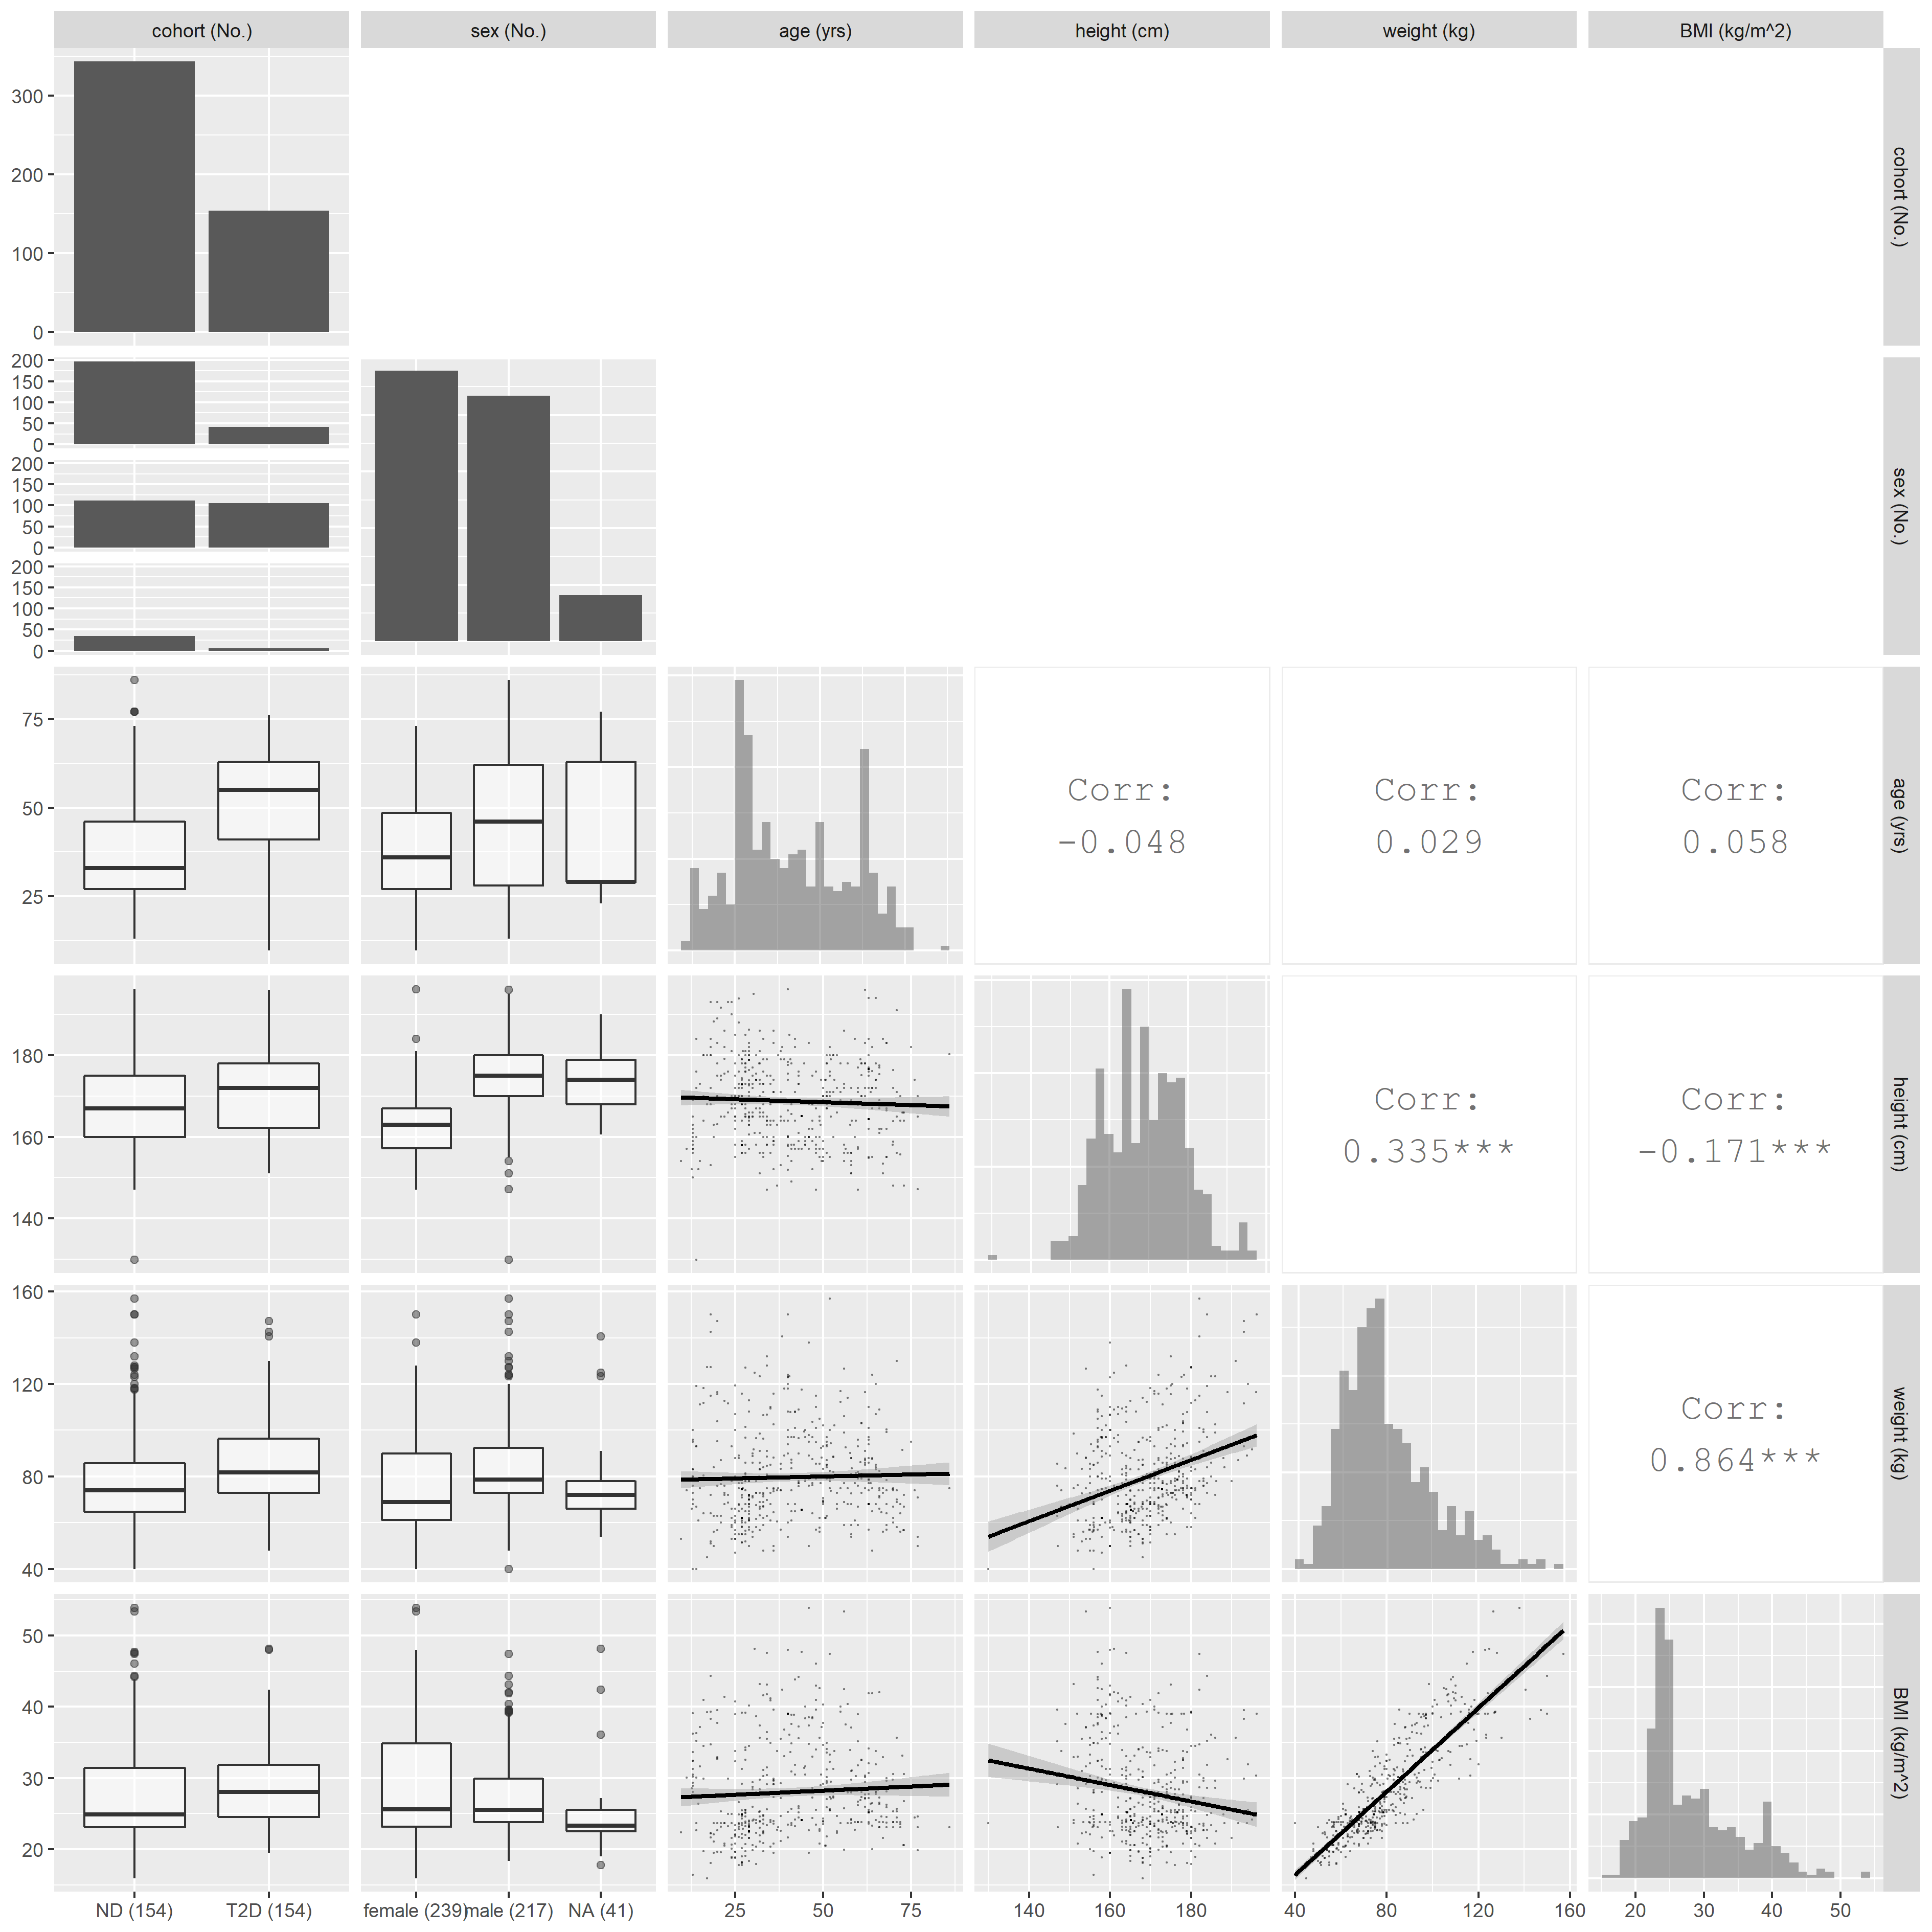
\includegraphics[width=15cm]{fig1.PNG}
\end{center}
\caption{Overview of covariate values and relationships. Histograms plots for continuous covariates and bar graphs for discrete covariates are shown on the diagnoal. In the lower triangle, the boxplots between continuous and discrete covariates and scatter plots between continuous covariates are displayed. In the upper triangle, the correlation coefficients between continuous covariates are shown}
\label{fig: cova}
\end{figure}

\begin{figure}[h!]
\begin{center}
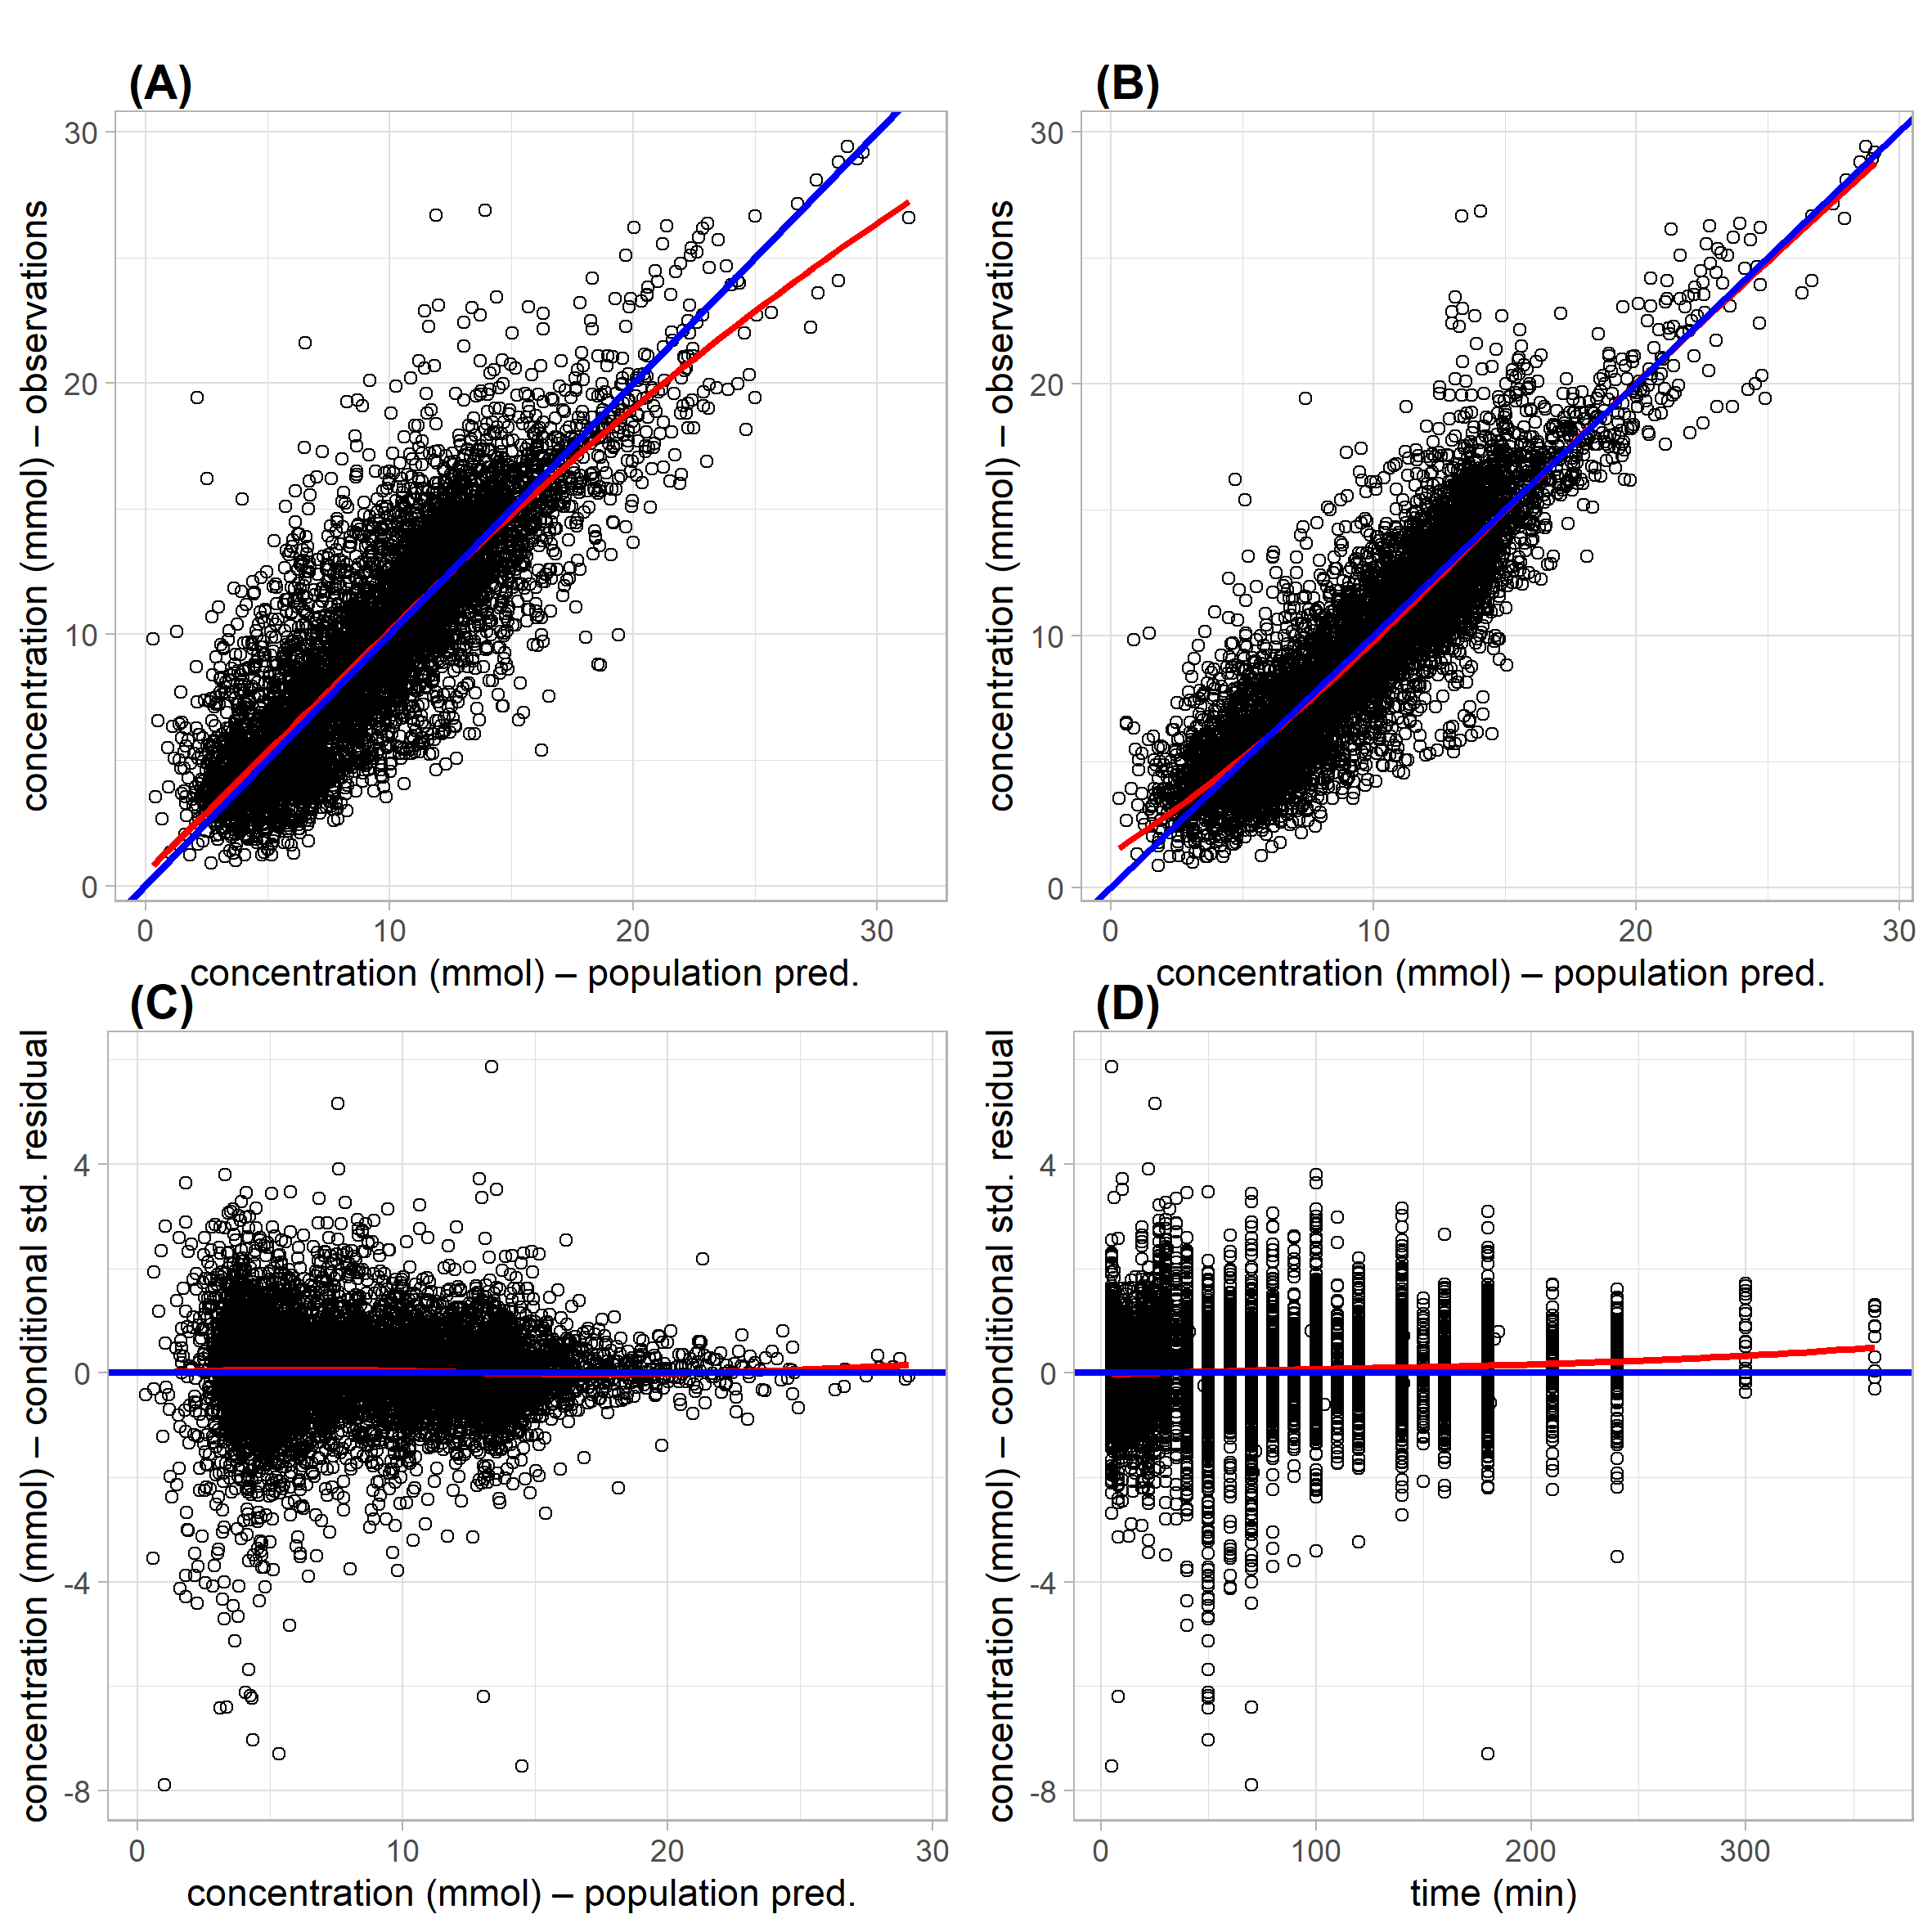
\includegraphics[width=15cm]{fig2.PNG}
\end{center}
\caption{Goodness-of-fit plots of the base model without covariates and the final model with covariates. \textbf{(A)}: observed glucose concentration versus population prediction from the base model. \textbf{(B)}: observed glucose concentration versus population prediction from the final model. \textbf{(C)}: conditional standardized residuals versus population prediction in  the final model. \textbf{(D)}: conditional standardized residual in the final model versus time. Blue lines are the lines of identity or zero value; red lines are loess smooth curves}
\label{fig: fittings}
\end{figure}

\begin{figure}[h!]
\begin{center}
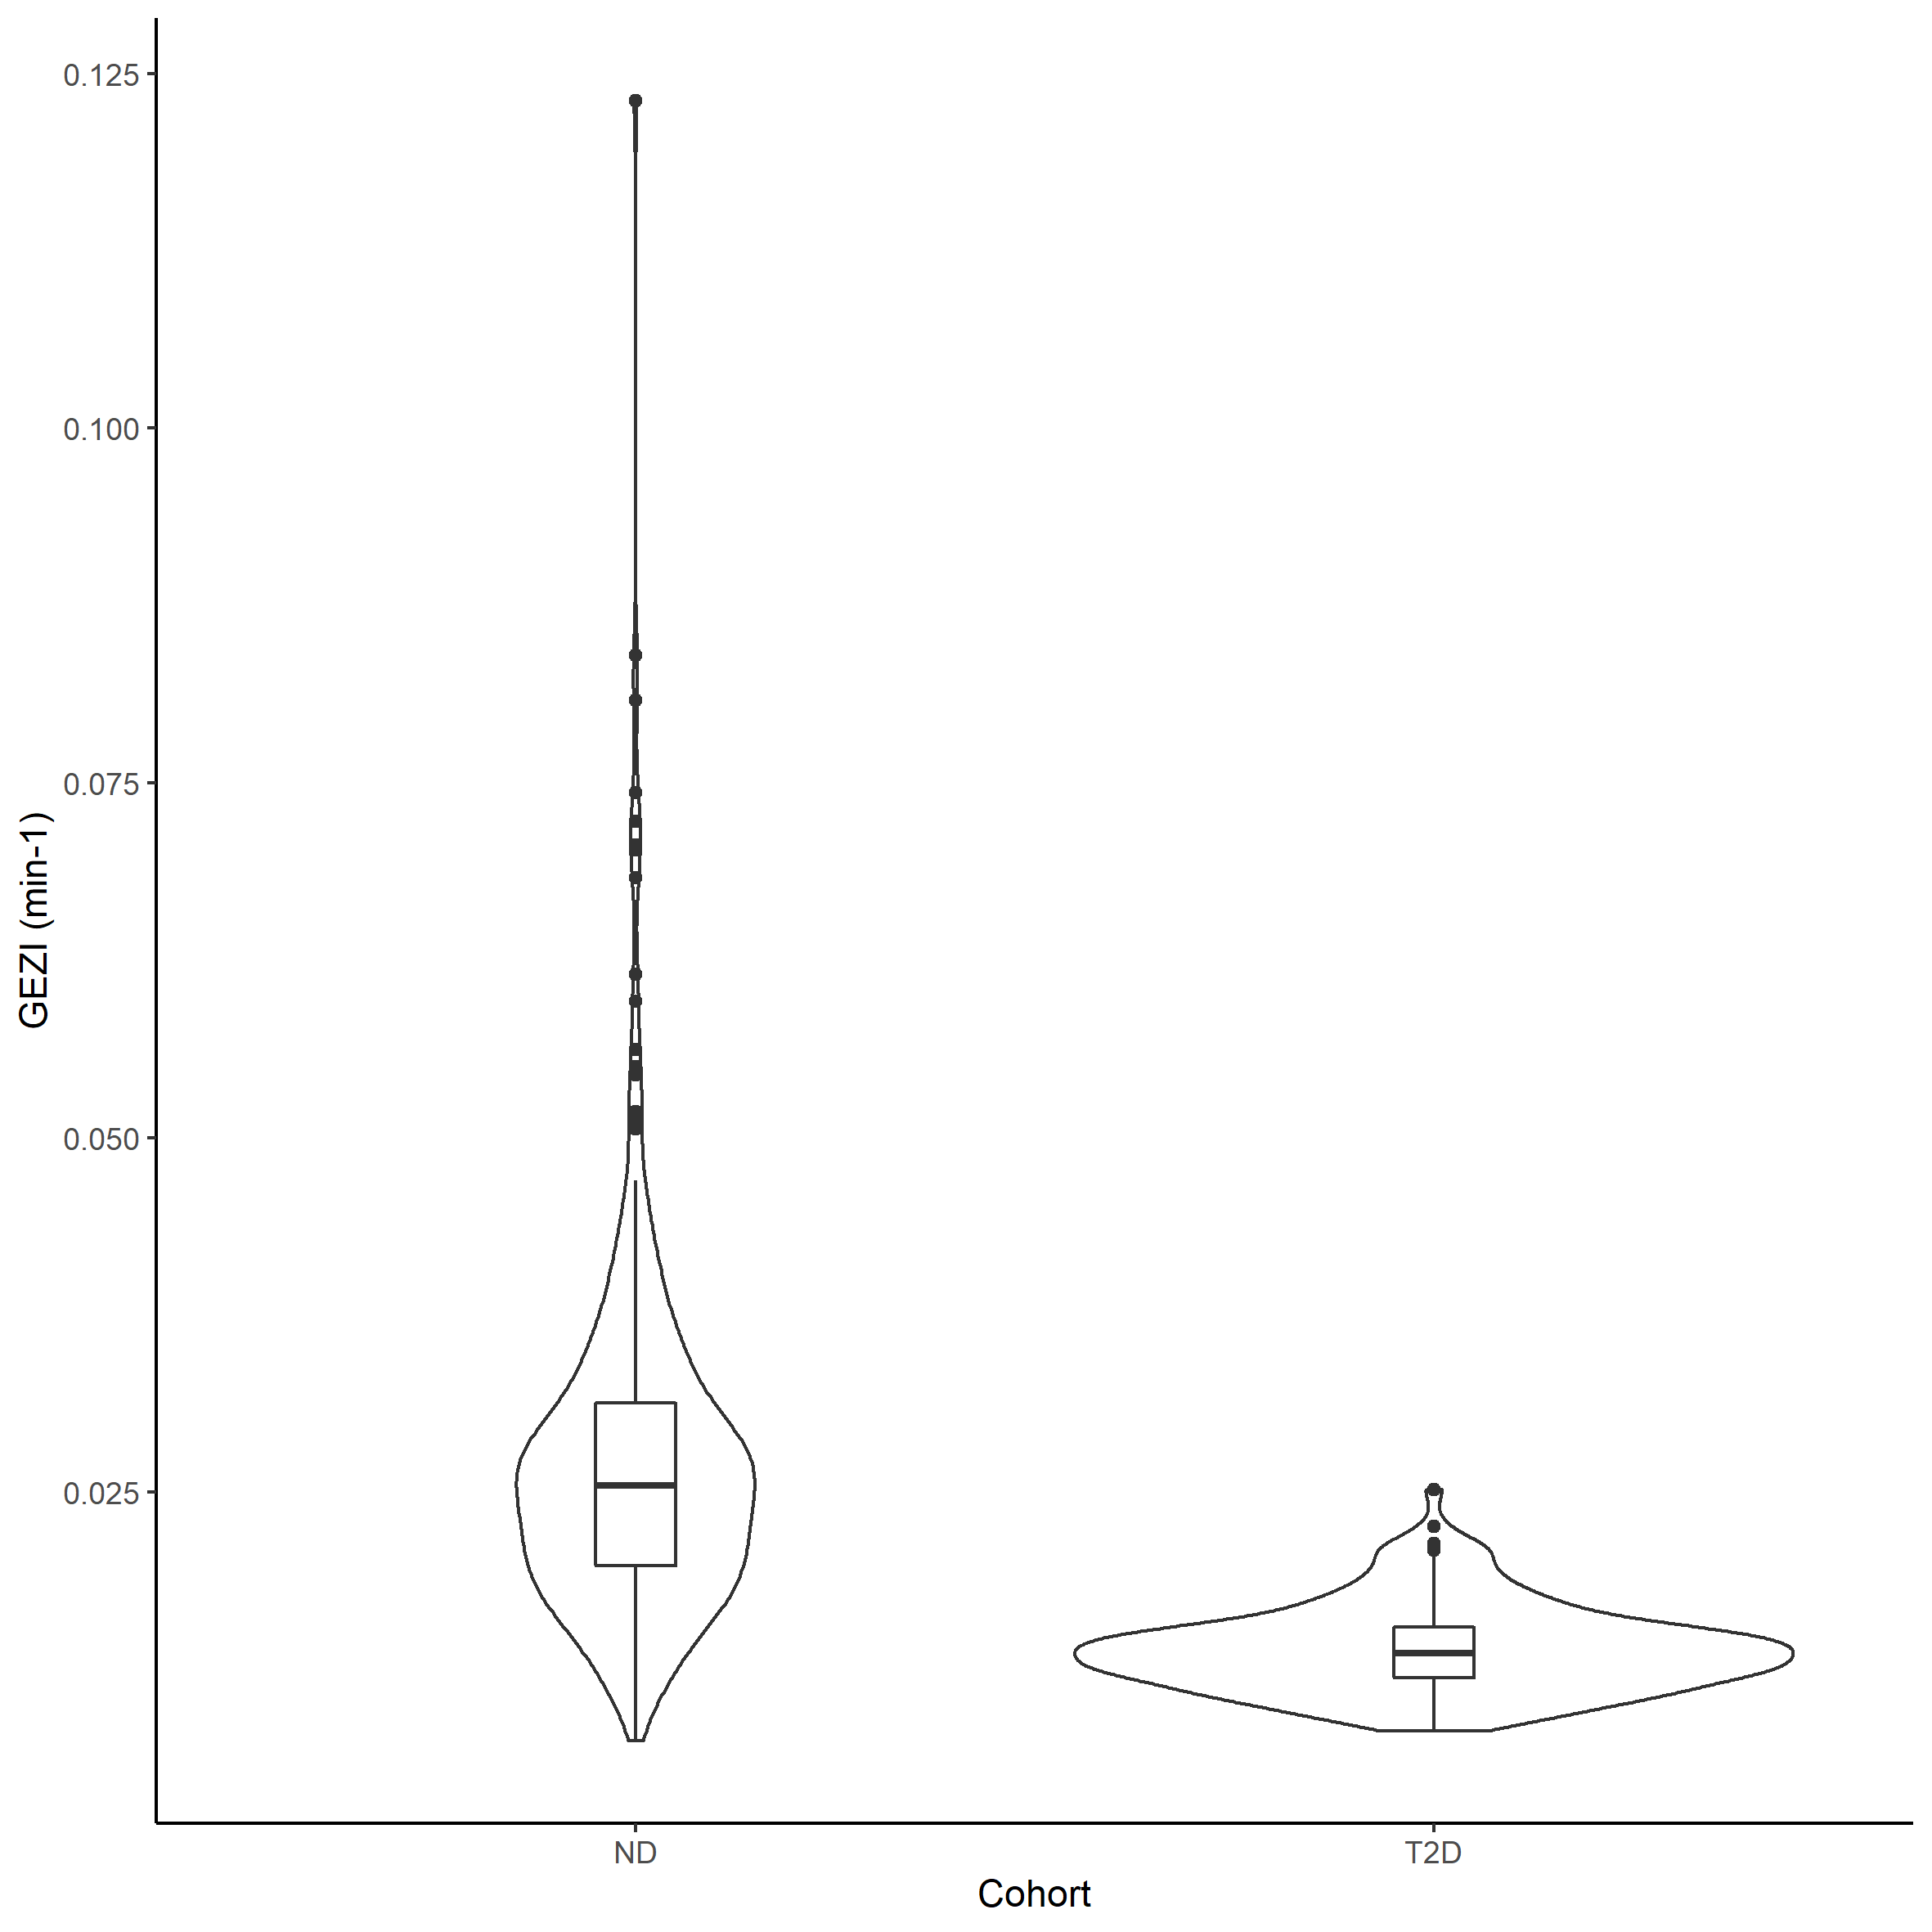
\includegraphics[width=15cm]{fig3.PNG}
\end{center}
\caption{Violin plots showing the distribution of the individual subjects conditional mean estimates of $GEZI$ in the ND and T2D cohorts. Boxplots were inserted for each cohort to indicate medians and interquartile ranges}
\label{fig: SG_co}
\end{figure}

\begin{figure}[h!]
\begin{center}
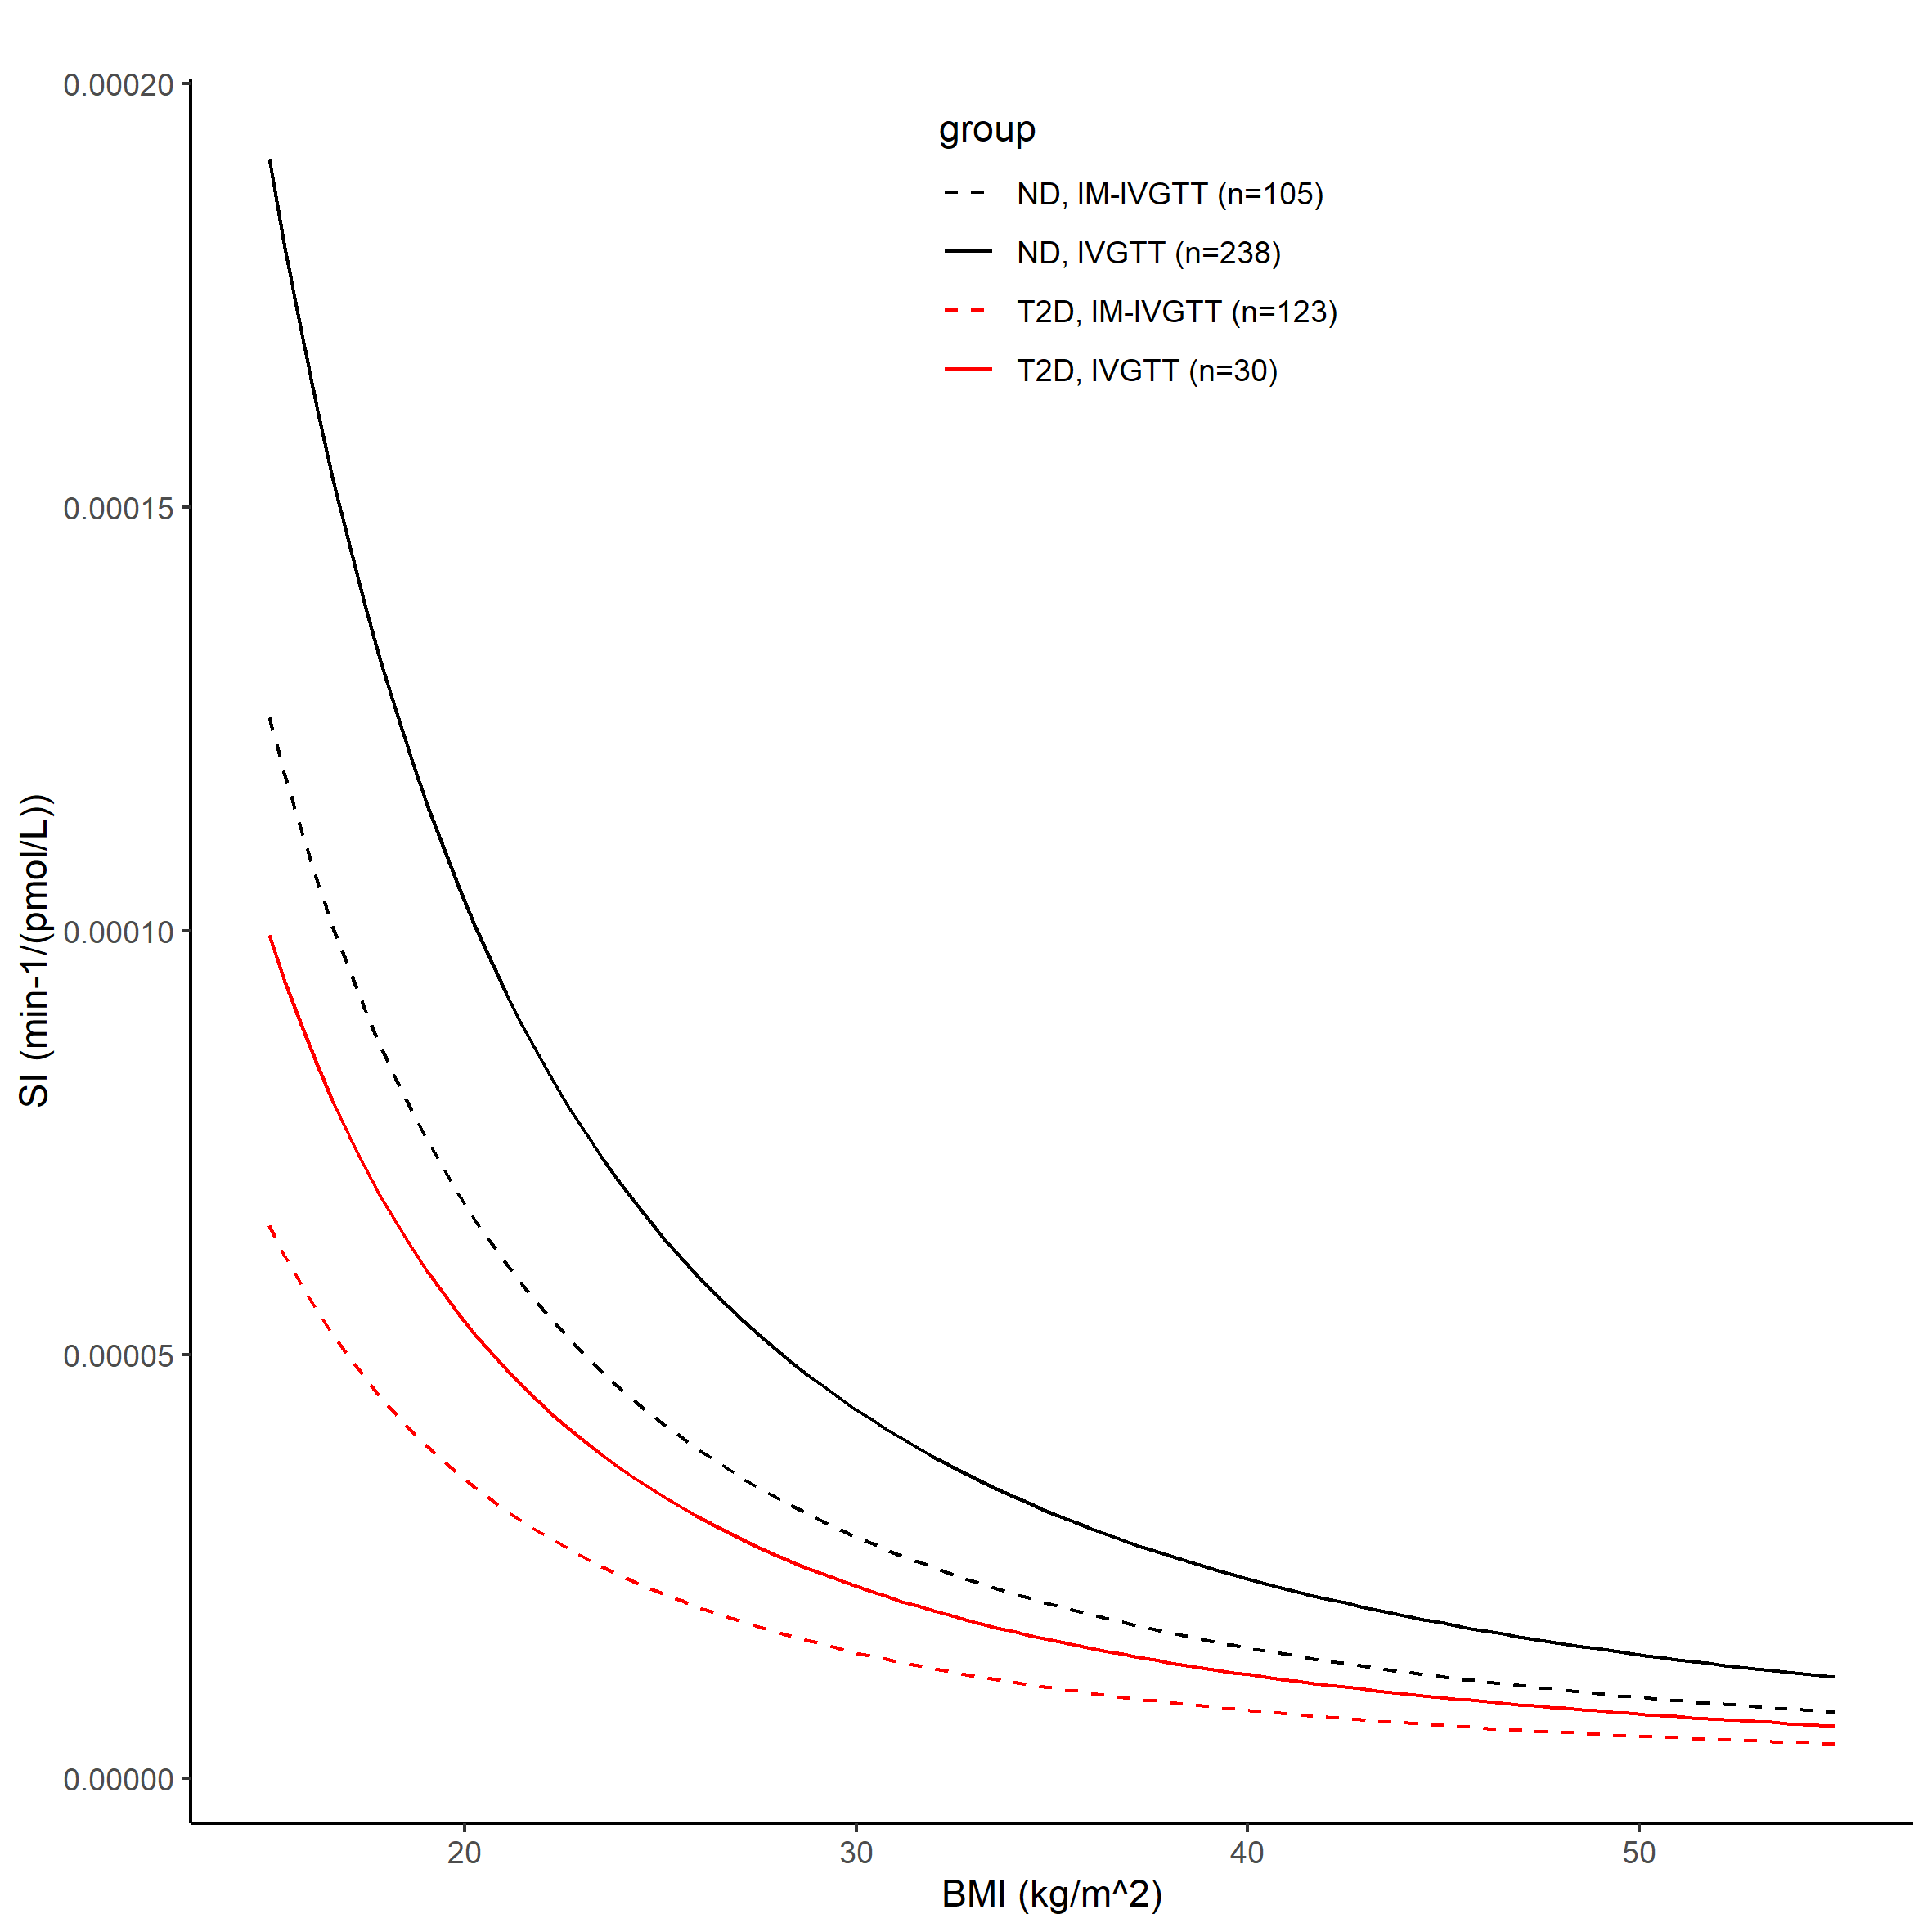
\includegraphics[width=15cm]{fig4.PNG}
\end{center}
\caption{The black lines show the covariate model prediction of the typical value of $S_I$ versus BMI in ND subjects, with the solid line indicating subjects in IVGTT and dash line indicating IM-IVGTT. The red lines are the corresponding curves in T2D patients}
\label{fig: SI_BMI}
\end{figure}

\begin{figure}[h!]
\begin{center}
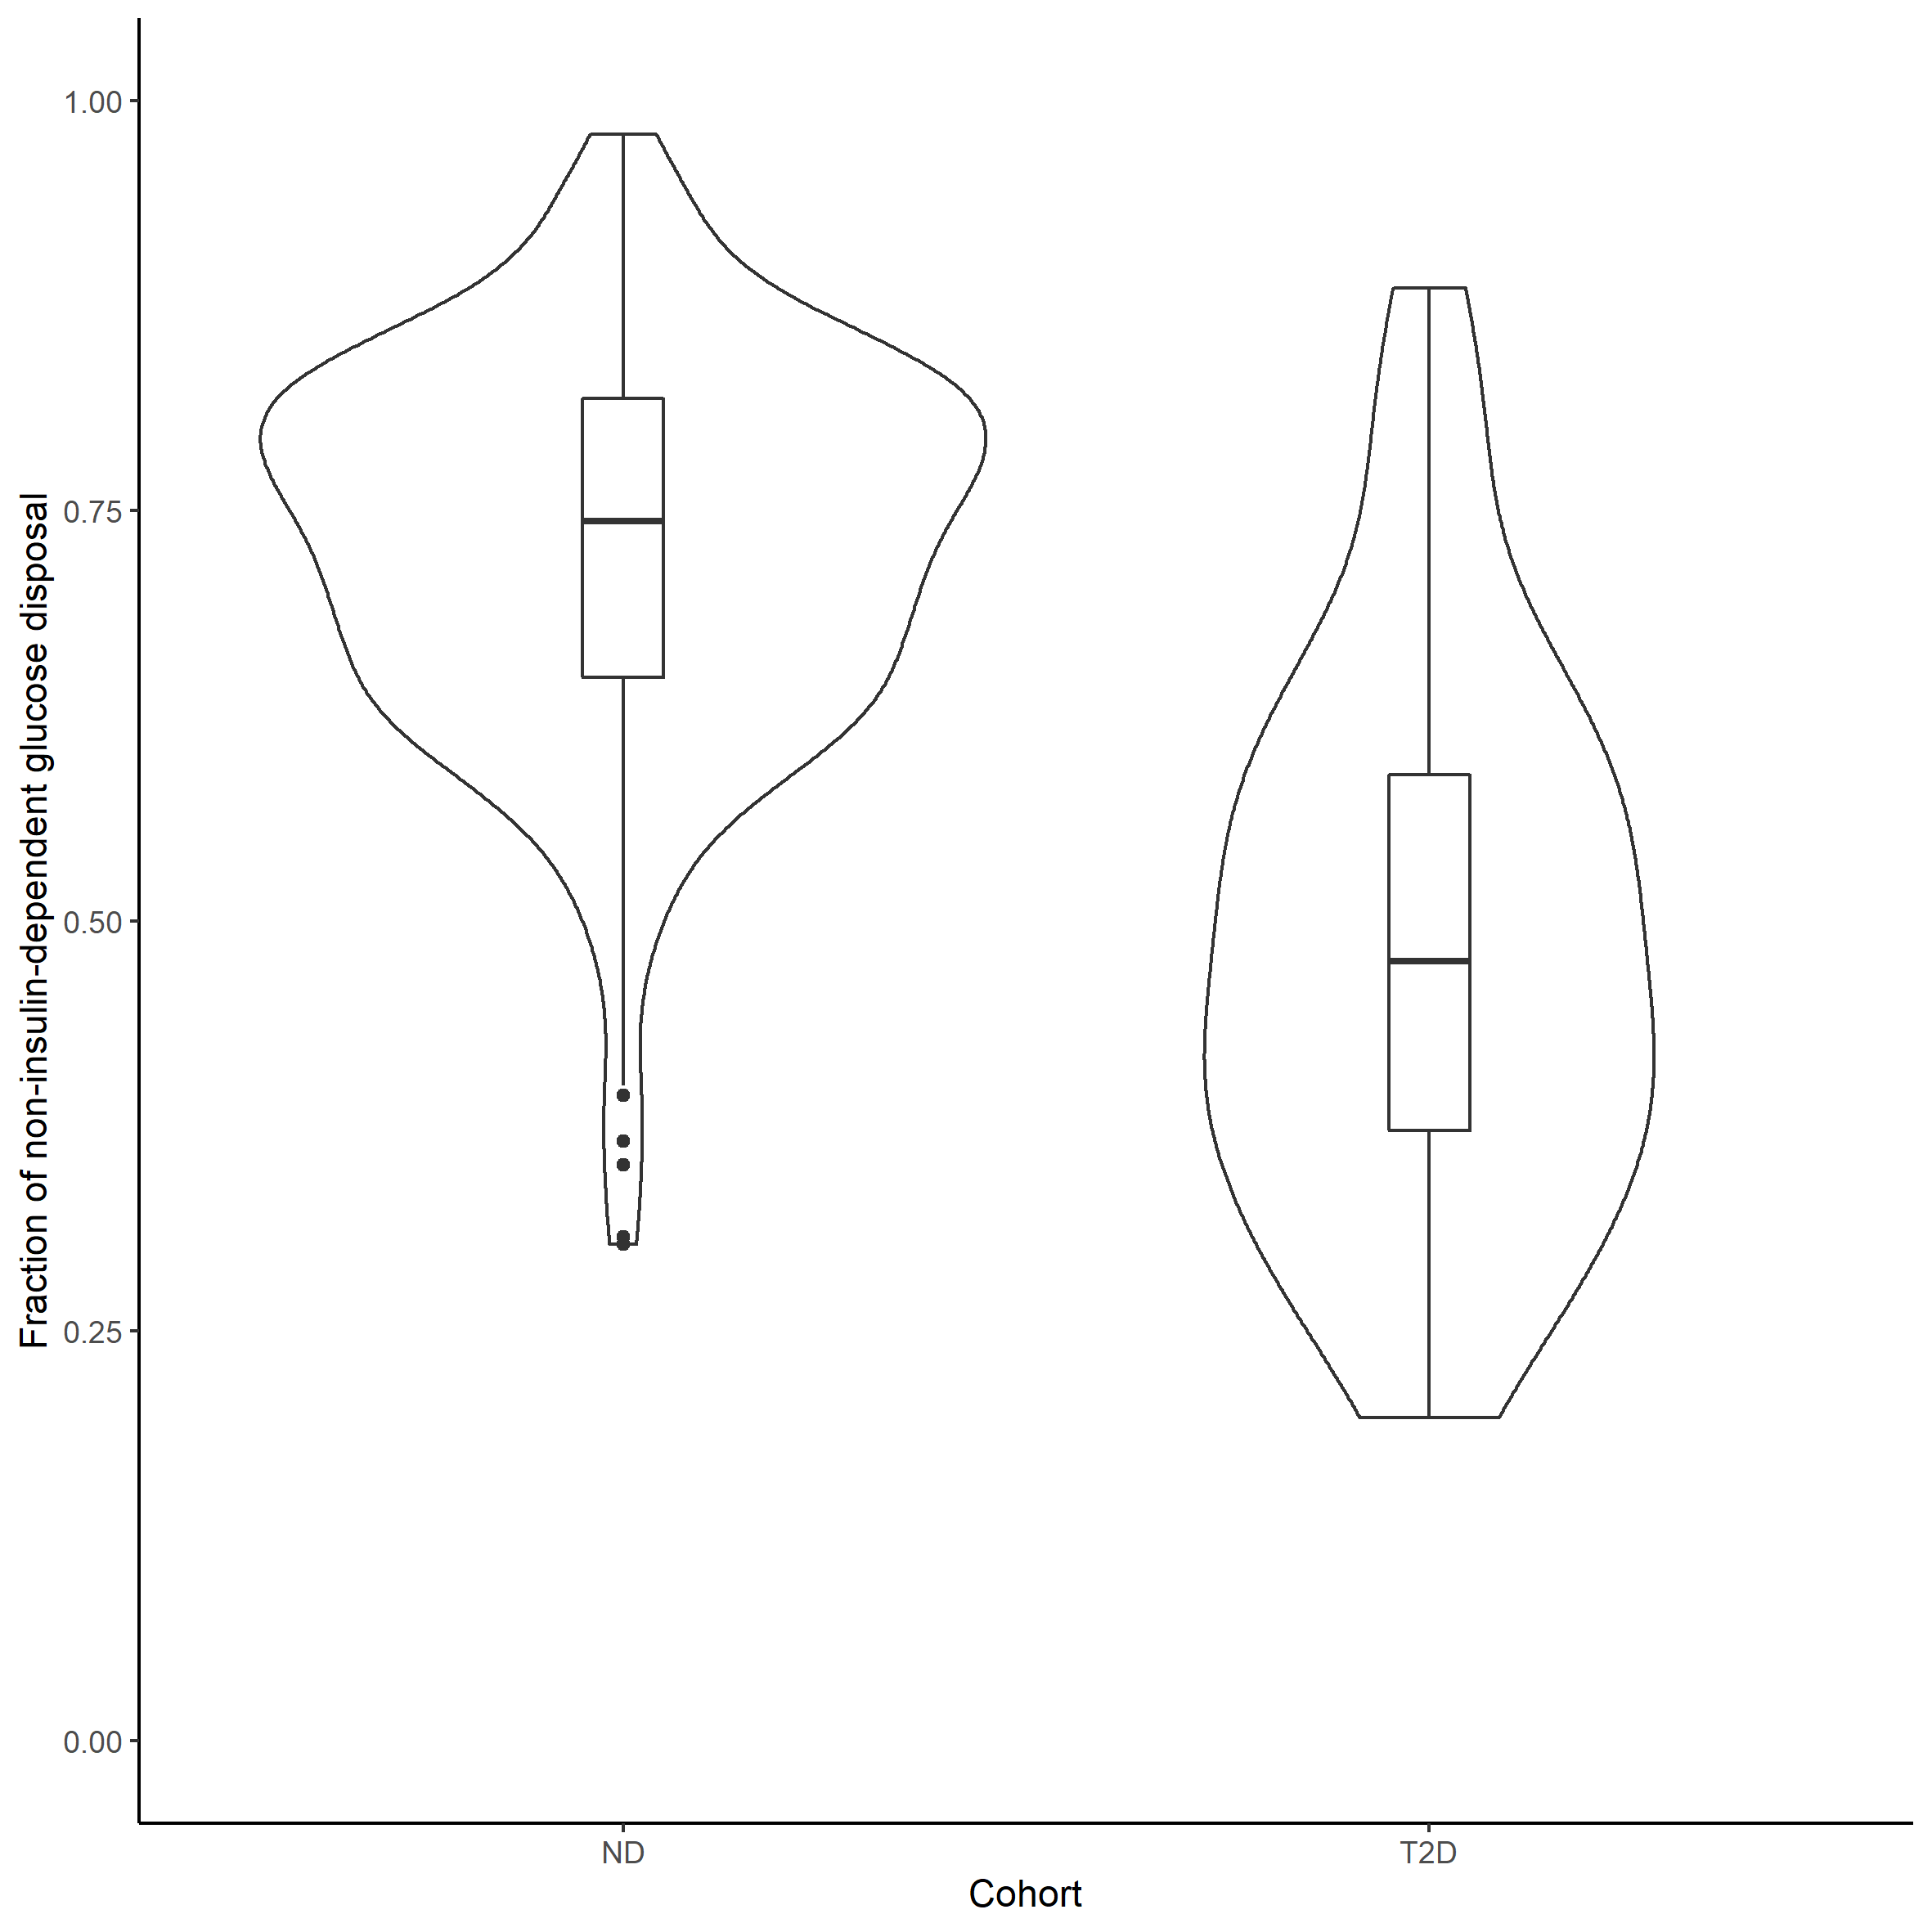
\includegraphics[width=15cm]{fig5.PNG}
\end{center}
\caption{Violin plots showing the distribution of the fraction of non–insulin-dependent net glucose disposal in 238 ND subjects and 30 T2D patients that underwent an IVGTT test. Boxplots were inserted for each cohort to indicate medians and interquartile ranges}
\label{fig: frac}
\end{figure}

\end{document}


